\documentclass[10pt,a4paper]{article}   
\usepackage[utf8]{inputenc}
\usepackage[T1]{fontenc}
\usepackage[top=0.68in,bottom=0.68in,left=0.70in,right=0.70in]{geometry}
\usepackage{graphicx}
\usepackage{booktabs}
\usepackage{array}
\usepackage{longtable}
\usepackage{multirow}
\usepackage{makecell}
\usepackage{tabularx}
\usepackage{colortbl}
\usepackage{xcolor}
\usepackage{hyperref}
\usepackage{url}
\usepackage{amsmath}
\usepackage{amssymb}
\usepackage{enumitem}
\usepackage{caption}
\usepackage{subcaption}
\usepackage{float}
\usepackage{morefloats} 
\usepackage{pgfplots}
\usepackage{tikz}
\usetikzlibrary{shapes.geometric, arrows, positioning, calc, fit, backgrounds}
\pgfplotsset{compat=1.17}
\usepackage{setspace}
\usepackage{microtype}
\usepackage{titlesec}
\usepackage{fancyhdr}
\usepackage{dblfloatfix}
\usepackage{pdflscape}
\setcounter{topnumber}{4}
\setcounter{dbltopnumber}{4}
\renewcommand{\topfraction}{0.9}
\renewcommand{\dbltopfraction}{0.9}
\renewcommand{\textfraction}{0.07}
\setstretch{1.0}
\setlength{\columnsep}{0.28in}
\setlength{\parindent}{1em}
\setlength{\parskip}{0pt}
\setlength{\headheight}{12pt}
\titleformat{\section}{\normalfont\small\bfseries}{\thesection.}{0.45em}{}
\titleformat{\subsection}{\normalfont\small\itshape}{\thesubsection.}{0.45em}{}
\titleformat{\subsubsection}{\normalfont\footnotesize\itshape}{\thesubsubsection.}{0.45em}{}
\titlespacing*{\section}{0pt}{1.1ex plus 0.3ex minus 0.2ex}{0.6ex}
\titlespacing*{\subsection}{0pt}{0.9ex plus 0.2ex minus 0.2ex}{0.45ex}
\titlespacing*{\subsubsection}{0pt}{0.75ex plus 0.2ex minus 0.1ex}{0.35ex}
\captionsetup{font=footnotesize,labelfont=bf,labelsep=period,skip=4pt}
\pagestyle{fancy}
\fancyhf{}
\fancyhead[L]{\scriptsize\thepage}
\fancyhead[C]{\scriptsize M. I. A. Khan et al. / Systematic Literature Review on LLM Code Generation}
\renewcommand{\headrulewidth}{0pt}
\hypersetup{
    colorlinks=true,
    linkcolor=blue,
    filecolor=magenta,
    urlcolor=blue,
    citecolor=blue
}
\definecolor{headerblue}{RGB}{31,78,120}
\definecolor{lightgray}{RGB}{240,240,240}

\newenvironment{topminipage}[1]{\begin{minipage}[t]{#1}}{\end{minipage}}

\title{\textbf{A Systematic Literature Review on Large Language Model-Based \\
Code Generation: Bug Taxonomy, Verification, and \\
Iterative Self-Repair}}
\author{
Muhmmad Immad Ahmed Khan, Adan Shahzad, Zikria Akhtar, Mudassar Adeel  \\
\small Capital University of Science and Technology, Islamabad, Pakistan \\
}
\date{\today}
\begin{document}
\twocolumn[
\thispagestyle{empty}
\begingroup
\setstretch{1.0}
\noindent{\raggedright\fontsize{17}{20}\selectfont\bfseries
A Systematic Literature Review on Large Language Model-Based Code Generation:\\
Bug Taxonomy, Verification, and Iterative Self-Repair\par}
\vspace{0.55em}

\noindent{\large Muhmmad Immad Ahmed Khan\textsuperscript{a},
Adan Shahzad\textsuperscript{a}, Zikria Akhtar\textsuperscript{a},
Mudassar Adeel\textsuperscript{a}\par}
\vspace{0.25em}
\noindent{\small\itshape
\textsuperscript{a}Capital University of Science and Technology, Islamabad, Pakistan\par}
\vspace{0.9em}
\hrule height 0.6pt
\vspace{0.8em}

%====================================================================
% ABSTRACT
%====================================================================
\noindent
\begin{topminipage}{0.25\textwidth}
\vspace{0pt}
{\small\bfseries\textls{ARTICLE INFO}\par}
\vspace{0.45em}
\hrule height 0.35pt
\vspace{0.55em}
{\fontsize{8}{9.4}\selectfont
\textit{Article type:}\par
Systematic Literature Review\par
\vspace{0.65em}
\textit{Manuscript status:}\par
In preparation\par
\vspace{0.8em}
\hrule height 0.35pt
\vspace{0.55em}
\textit{Review window:}\par
2021--2025\par
\vspace{0.8em}
\textit{Keywords:}\par
Large language models\par
Code generation\par
Bug taxonomy\par
Verification\par
Iterative self-repair\par
Automated program repair\par}
\end{topminipage}\hfill
\begin{topminipage}{0.70\textwidth}
\vspace{0pt}
{\small\bfseries\textls{ABSTRACT}\par}
\vspace{0.45em}
\hrule height 0.35pt
\vspace{0.5em}
{\fontsize{8.2}{9.7}\selectfont
\noindent
The rapid advancement of Large Language Models (LLMs) has transformed automated code generation, yet LLM-generated code continues to exhibit syntactic errors, runtime failures, functional bugs, and security vulnerabilities. Contemporary responses to these shortcomings span structured prompting, verification through test execution and static analysis, and iterative self-repair grounded in execution feedback. However, these research threads have largely evolved in isolation, and no systematic synthesis exists that unifies code generation, bug taxonomy construction, verification, and bounded iterative repair within a single-agent pipeline perspective.
\noindent
This Systematic Literature Review (SLR) aims to identify, classify, and analyze the latest research practices from the 2021--2025 search window, including studies retained under the search protocol and formally published in 2026, where LLM-based approaches have been utilized for code generation, bug detection and classification, verification and test generation, iterative self-repair, efficiency optimization, and security assurance. The review further investigates the tools, frameworks, and benchmarks employed, and highlights research gaps that motivate the development of a single-agent generate--verify--repair framework with taxonomy-guided feedback and a bounded iteration budget, extending the empirical foundation established by Dou et al.
\noindent
Systematic Literature Review methodology has been adopted following the guidelines proposed by Kitchenham, as operationalized by Rashid et al. A comprehensive review protocol was developed incorporating six concrete selection criteria, a structured search process across four renowned scientific databases (IEEE, ACM, Springer, Elsevier, supplemented by arXiv), quality assessment procedures, and a formal data extraction and synthesis framework. Six predefined categories guided the classification of selected research works.
\noindent
From an initial pool of 8,500 gross retrievals (pre-deduplication) across five sources (IEEE, ACM, Springer, Elsevier, arXiv), 46 primary research works were selected through a purposive screening process guided by six selection criteria, continued until thematic saturation was reached across the six target categories. The selected studies were classified into six categories: General (8), Code Generation (8), Bug Detection \& Classification (4), Verification \& Test Generation (10), Iterative Self-Repair (10), and Optimization \& Security (9). The analysis identified zero-shot prompting as the most prevalent prompting technique family (37.0\% of studies), self-critique with compiler or execution feedback as the leading repair mechanism (19.6\%), and compiler or execution feedback as the dominant repair feedback source, while iteration budgets across the literature were found to be predominantly post-hoc or unbounded, with only a minority adopting fixed small budgets ($\leq$3 iterations). The bug-taxonomy synthesis is anchored by the fine-grained taxonomies of Dou et al.~\cite{dou2026}, Tambon et al.~\cite{tambon2025}, Wang et al.~\cite{wang2025where}, and Pan et al.~\cite{pan2024lost}. HumanEval/MBPP/APPS were the most widely used benchmarks. A comprehensive comparative evaluation of 39 tools and frameworks was performed using both general and activity-specific characteristics, including feedback source, verification signal, oracle assumption, and iteration budget.
\noindent
The SLR reveals that contemporary research treats verification and repair as separable concerns, with bug-taxonomy knowledge, verification signals, and iteration budgets rarely integrated into one repair loop. A significant research gap exists in single-agent frameworks that couple fine-grained bug-taxonomy-guided feedback with verification-driven, bounded-iteration self-repair. This gap justifies the development of a generate--verify--repair pipeline that targets higher repair success than the two-iteration baseline reported by Dou et al., at a fraction of the computational cost documented for multi-agent alternatives.
}
\end{topminipage}
\par\vspace{0.8em}
\hrule height 0.6pt
\vspace{0.75em}
\endgroup
]

%====================================================================
% SECTION 1 — INTRODUCTION  (mirrors Rashid et al. Section 1)
%====================================================================
\section{Introduction}
\label{sec:introduction}
Large Language Models (LLMs) such as GPT-4, Claude-3, DeepSeek-V3/R1, Code Llama, and StarCoder-2 have fundamentally reshaped the landscape of automated software engineering. Modern LLM-based code generation systems achieve unprecedented performance on standard benchmarks, with reasoning-specialized models such as DeepSeek-R1 attaining up to 77.9\% pass rates on real-world programming tasks \cite{dou2026}. However, despite this remarkable progress, LLM-generated code continues to exhibit critical shortcomings, including syntax violations, runtime exceptions, functional bugs, inefficient algorithmic implementations, and security vulnerabilities \cite{bruni2025,liu2025llm4tdg}. The major LLM-based code generation activities considered in this review are shown in Fig.~\ref{fig:activities}.

Code generation from a natural language specification is the foremost activity. All subsequent activities (i.e., verification, repair, optimization, and security assurance) operate on the generated program. Verification is performed to establish whether the generated code satisfies its specification, typically through compiler checks, test execution, LLM-generated tests, runtime instrumentation, static analysis, or deductive formal verification~\cite{chen2023selfdebug,liu2025llm4tdg,sun2024clover}. If the code does not satisfy the verification requirements, corrections are made through iterative self-repair, in which the model revises its own output using the verification feedback, as shown in Fig.~\ref{fig:activities}. The final validated code is then evaluated against established benchmarks.

% ------- Fig 1: Major LLM-based code generation activities (Rashid Fig. 1 analog) -------
\begin{figure*}[!t]
\centering
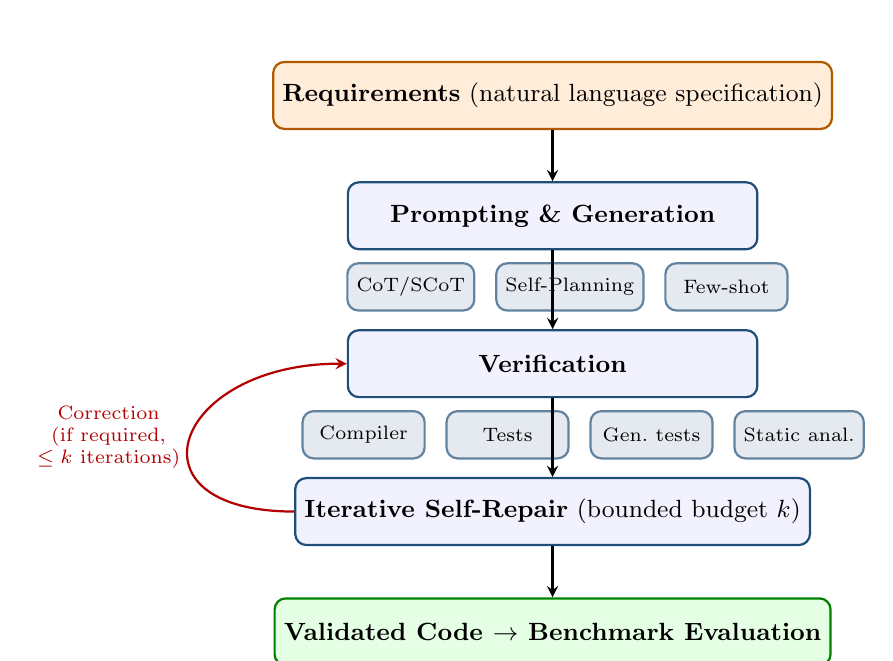
\begin{tikzpicture}[
    node distance=0.65cm,
    stage/.style={rectangle, rounded corners, draw=headerblue, thick,
        minimum width=5.2cm, minimum height=0.85cm, align=center,
        fill=blue!5, font=\small},
    substage/.style={rectangle, rounded corners, draw=headerblue!70, thick,
        minimum width=1.55cm, minimum height=0.6cm, align=center,
        fill=headerblue!12, font=\scriptsize},
    arrow/.style={-stealth, thick},
    loop/.style={-stealth, thick, red!70!black}
]
\node[stage, fill=orange!15, draw=orange!70!black] (req) {\textbf{Requirements} (natural language specification)};
\node[stage, below=of req] (gen) {\textbf{Prompting \& Generation}};
\node[substage, below=0.15cm of gen, xshift=-1.8cm] (cot) {CoT/SCoT};
\node[substage, right=0.25cm of cot] (plan) {Self-Planning};
\node[substage, right=0.25cm of plan] (fs) {Few-shot};
\node[stage, below=1.0cm of gen] (ver) {\textbf{Verification}};
\node[substage, below=0.15cm of ver, xshift=-2.4cm] (comp) {Compiler};
\node[substage, right=0.25cm of comp] (test) {Tests};
\node[substage, right=0.25cm of test] (gtest) {Gen.\ tests};
\node[substage, right=0.25cm of gtest] (sa) {Static anal.};
\node[stage, below=1.0cm of ver] (rep) {\textbf{Iterative Self-Repair} (bounded budget $k$)};
\node[stage, below=of rep, fill=green!10, draw=green!50!black] (final) {\textbf{Validated Code $\rightarrow$ Benchmark Evaluation}};
\draw[arrow] (req) -- (gen);
\draw[arrow] (gen) -- (ver);
\draw[arrow] (ver) -- (rep);
\draw[arrow] (rep) -- (final);
\draw[loop] (rep.west) .. controls +(-2.2,0) and +(-2.2,0) .. (ver.west)
    node[midway, left, align=center, font=\scriptsize\color{red!70!black}]
    {Correction\\(if required,\\$\leq k$ iterations)};
\end{tikzpicture}
\caption{Major LLM-based code generation activities in a single-agent generate--verify--repair pipeline.}
\label{fig:activities}
\end{figure*}

Although researchers have put substantial effort into LLM-based code generation, it remains a challenging area due to the diversity of bug types exhibited by generated code \cite{dou2026}. It is always difficult to select appropriate prompting techniques and reasoning scaffolds for a given task. Moreover, there is a considerable dependency among the different activities (i.e., generation, verification, repair, optimization, and security assurance) that requires sufficient knowledge of all phases. Similarly, there are separate tools, feedback mechanisms, and benchmarks for each activity, and the selection of an appropriate verification signal and repair strategy is always problematic for researchers and practitioners. Notably, while multi-agent frameworks such as ChatDev, MetaGPT, AutoGen, AnnCoder, and Bai et al.~\cite{qian2023chatdev,hong2023metagpt,wu2023autogen,zhang2025anncoder,bai2025collab} have attracted considerable attention, their documented computational overheads motivate a systematic examination of what disciplined \textit{single-agent} pipelines can achieve when generation is coupled with explicit verification and bounded iterative repair.

Keeping in view the current state of affairs, the objective of this systematic literature review (SLR) is to identify the latest research practices where LLM-based approaches have been used for code generation, verification, and self-repair. The identified researches are classified into six categories depending upon their relevance with the corresponding activity. Furthermore, various tools, frameworks, and benchmarks have also been identified. Consequently, the following research questions have been developed for this SLR:

\textbf{Research question 1:} What important researches have been reported from 2021 to 2025 where LLM-based approaches have been utilized to support code generation, bug detection and classification, verification and test generation, iterative self-repair, efficiency optimization, and security assurance?

\textbf{Research question 2:} Which prompting and reasoning techniques (zero-shot, few-shot, Chain-of-Thought, Structured Chain-of-Thought, Self-Planning, Recursive Criticism and Improvement, self-critique) are more frequently utilized for LLM-based code generation during 2021--2025 researches?

\textbf{Research question 3:} Which verification and self-repair mechanisms (compiler/execution feedback, LLM-generated test verification, runtime-trace debugging, static analysis integration, bug-taxonomy-guided repair, constraint-based reasoning, post-hoc candidate ranking) are more frequently utilized during 2021--2025 researches, and with what iteration budgets?

\textbf{Research question 4:} What are the significant tools, frameworks, and benchmarks for generation, verification, repair, optimization, and security in the context of LLM-based code generation, and how can they be compared based on general and activity-specific characteristics (including feedback source, verification signal, oracle assumption, and iteration budget)?

The answers to all research questions are given in Section~\ref{sec:answers}. A review protocol, incorporating selection and rejection criteria, has been developed to perform this SLR. We have defined six categories (Section~\ref{sec:categories}) for the selected researches in order to obtain the answers to our research questions. A complete overview of this research work is presented in Fig.~\ref{fig:overview}.

A review protocol is developed (Section~\ref{sec:protocol}) that contains the selection and rejection criteria (Section~\ref{sec:criteria}). As shown in Fig.~\ref{fig:overview}, four scientific databases plus arXiv are selected for the search process (Section~\ref{sec:search_process}) and six categories are defined (Section~\ref{sec:categories}) to classify the 46 selected researches. Similarly, data extraction elements (Section~\ref{sec:data_extraction}) are defined to perform comprehensive analysis and synthesis of the selected researches. Consequently, the major findings of the SLR are summarized in Section~\ref{sec:results}. On the basis of the SLR, we preliminarily identify 39 tools (Section~\ref{sec:tools_prelim}) that have been used in the selected researches to perform particular activities. In Section~\ref{sec:tools_investigation}, various tools characteristics (Section~\ref{sec:char_defined}) are defined for further evaluation. Results in Sections~\ref{sec:results} and \ref{sec:tools_investigation} provide the answers to the research questions, which are discussed in Section~\ref{sec:answers}. Further important aspects, the research gap, and certain limitations are discussed in Section~\ref{sec:discussion}. Finally, Section~\ref{sec:conclusions} concludes the article.

% ------- Fig 2: Overview of research (Rashid Fig. 2 analog) -------
\begin{figure*}[!t]
\centering
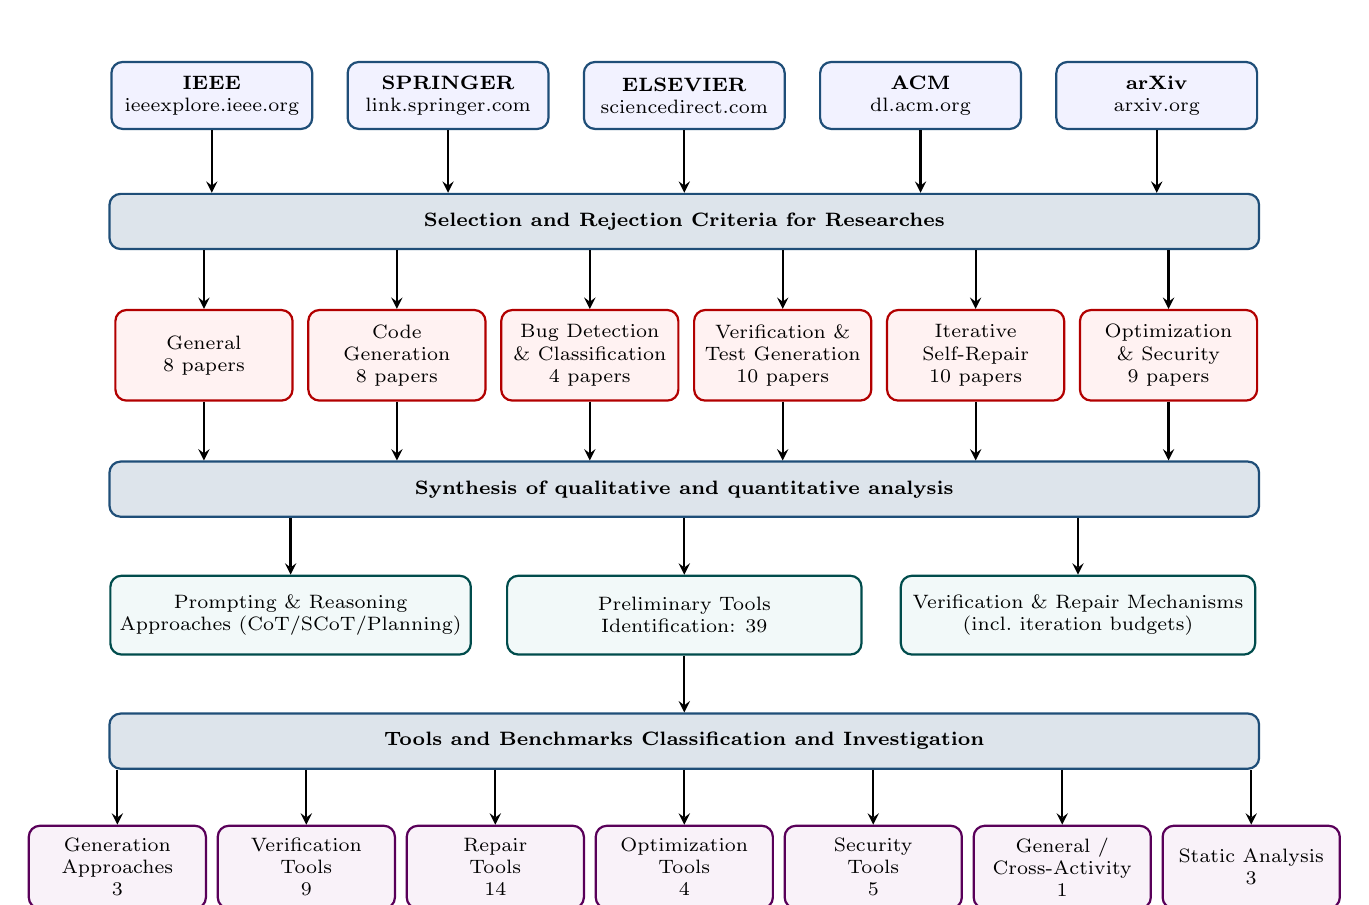
\begin{tikzpicture}[font=\scriptsize,
    db/.style={draw=headerblue, thick, fill=blue!5, rounded corners,
        minimum width=2.55cm, minimum height=0.85cm, align=center},
    bar/.style={draw=headerblue, thick, fill=headerblue!15, rounded corners,
        minimum width=14.6cm, minimum height=0.7cm, align=center, font=\scriptsize\bfseries},
    cat/.style={draw=red!70!black, thick, fill=red!5, rounded corners,
        minimum width=2.25cm, minimum height=1.15cm, align=center},
    outbox/.style={draw=teal!60!black, thick, fill=teal!5, rounded corners,
        minimum width=4.5cm, minimum height=1.0cm, align=center},
    tool/.style={draw=violet!70!black, thick, fill=violet!5, rounded corners,
        minimum width=2.25cm, minimum height=1.05cm, align=center, font=\scriptsize},
    arrow/.style={-stealth, thick}
]
% databases row
\node[db] (d1) at (-6.0,0) {\textbf{IEEE}\\ieeexplore.ieee.org};
\node[db] (d2) at (-3.0,0) {\textbf{SPRINGER}\\link.springer.com};
\node[db] (d3) at (0,0)    {\textbf{ELSEVIER}\\sciencedirect.com};
\node[db] (d4) at (3.0,0)  {\textbf{ACM}\\dl.acm.org};
\node[db] (d5) at (6.0,0)  {\textbf{arXiv}\\arxiv.org};
% criterion bar
\node[bar] (crit) at (0,-1.6) {Selection and Rejection Criteria for Researches};
% category row
\node[cat] (c1) at (-6.1,-3.3) {General\\ 8 papers};
\node[cat] (c2) at (-3.65,-3.3) {Code\\Generation\\ 8 papers};
\node[cat] (c3) at (-1.2,-3.3) {Bug Detection\\\& Classification\\ 4 papers};
\node[cat] (c4) at (1.25,-3.3) {Verification \&\\Test Generation\\ 10 papers};
\node[cat] (c5) at (3.7,-3.3) {Iterative\\Self-Repair\\ 10 papers};
\node[cat] (c6) at (6.15,-3.3) {Optimization\\\& Security\\ 9 papers};
% synthesis bar
\node[bar] (syn) at (0,-5.0) {Synthesis of qualitative and quantitative analysis};
% outcomes row
\node[outbox] (o1) at (-5.0,-6.6) {Prompting \& Reasoning\\Approaches (CoT/SCoT/Planning)};
\node[outbox] (o2) at (0,-6.6)    {Preliminary Tools\\Identification: 39};
\node[outbox] (o3) at (5.0,-6.6)  {Verification \& Repair Mechanisms\\(incl.\ iteration budgets)};
% classification bar
\node[bar] (cls) at (0,-8.2) {Tools and Benchmarks Classification and Investigation};
% tool categories row
\node[tool] (t1) at (-7.2,-9.8) {Generation\\Approaches\\ 3};
\node[tool] (t2) at (-4.8,-9.8) {Verification\\Tools\\ 9};
\node[tool] (t3) at (-2.4,-9.8) {Repair\\Tools\\ 14};
\node[tool] (t4) at (0,-9.8)    {Optimization\\Tools\\ 4};
\node[tool] (t5) at (2.4,-9.8)  {Security\\Tools\\ 5};
\node[tool] (t6) at (4.8,-9.8)  {General /\\Cross-Activity\\ 1};
\node[tool] (t7) at (7.2,-9.8)  {Static Analysis\\ 3};
% arrows
\foreach \d in {d1,d2,d3,d4,d5} \draw[arrow] (\d.south) -- (crit.north -| \d.south);
\foreach \c in {c1,c2,c3,c4,c5,c6} \draw[arrow] (crit.south -| \c.north) -- (\c.north);
\foreach \c in {c1,c2,c3,c4,c5,c6} \draw[arrow] (\c.south) -- (syn.north -| \c.south);
\foreach \o in {o1,o2,o3} \draw[arrow] (syn.south -| \o.north) -- (\o.north);
\draw[arrow] (o2.south) -- (cls.north);
\foreach \t in {t1,t2,t3,t4,t5,t6,t7} \draw[arrow] (cls.south -| \t.north) -- (\t.north);
\end{tikzpicture}
\caption{Overview of research.}
\label{fig:overview}
\end{figure*}

%====================================================================
% SECTION 2 — RESEARCH METHODOLOGY  (mirrors Rashid et al. Section 2)
%====================================================================
\section{Research Methodology}
\label{sec:methodology}
Systematic literature review \cite{kitchenham2004} has been used to carry out this research, following the operationalization demonstrated by Rashid et al.~\cite{rashid2015}. It is a proper and replicable process to document pertinent details on a precise research area for reviewing and investigating all existing research related to the research questions. Consequently, this research incorporates five stages: 1) categories definition, 2) review protocol development, 3) selection and rejection criteria, 4) search process and quality assessment, and 5) data extraction and synthesis.

\subsection{Categories Definition}
\label{sec:categories}
We have defined six categories in order to organize the selected researches. This categorization significantly improves the accuracy of the answers to our research questions. The categories are mutually complementary; a study addressing three or more activities simultaneously is assigned to the \textit{General} category, whereas studies targeting a specific activity are assigned to the corresponding specialized category. The details of the categories are given below.

\subsubsection{General category}
\label{sec:cat_general}
This category contains research works where comprehensive solutions covering multiple LLM-based code generation activities (e.g., end-to-end pipelines spanning generation, verification, iterative repair, and evaluation) are proposed. Studies covering at least three of the six activity types are assigned to this category.

\subsubsection{Code generation category}
\label{sec:cat_generation}
This category includes research works primarily focused on improving the generation of code from natural language specifications through techniques such as prompt engineering, in-context learning, planning-based decomposition, structured reasoning, and retrieval augmentation. Such researches do not significantly contribute to verification, repair, optimization, or security aspects.

Benchmark/dataset papers are cited as Code Generation only when their primary task is single-shot generation; multi-activity or repair-focused benchmarks are cited in the General category, or cited benchmark-only in Table~\ref{tab:cmp_benchmarks} without a primary-study category slot.

\subsubsection{Bug detection and classification category}
\label{sec:cat_bugs}
This category encompasses research works that propose taxonomies, classification schemes, or empirical characterizations of bugs introduced by LLM-generated code. These studies typically construct bug datasets, analyze root causes, and provide empirical insights into the limitations of contemporary LLMs.

\subsubsection{Verification and test generation category}
\label{sec:cat_verification}
This category is dedicated to research works whose principal contribution is establishing \textit{whether generated code is correct} prior to (or independent of) any repair action. It includes LLM-generated test suites, dual execution agreement, learned verifiers, runtime instrumentation and tracing, constraint checking, and benchmark test-adequacy hardening. The verification signal produced by these works is the input upon which iterative self-repair operates; consequently, this category constitutes essential infrastructure for the repair loop depicted in Fig.~\ref{fig:activities}.

\subsubsection{Iterative self-repair category}
\label{sec:cat_repair}
This category contains research works proposing automated repair mechanisms in which a single model iteratively revises its own (or another model's) output using feedback such as compiler diagnostics, failing tests, execution traces, or natural language critique. Techniques include self-debugging, self-refinement, fault-aware editing, conversational repair, and sampling-with-ranking paradigms. Critical analyses of the self-repair paradigm itself are also assigned to this category.

\subsubsection{Optimization and security category}
\label{sec:cat_optsec}
This category encompasses research works addressing the efficiency, quality, readability, or maintainability of LLM-generated code, as well as its security dimension, including vulnerability detection, secure prompt engineering, CWE mitigation, and security-aware fine-tuning.

\subsection{Review Protocol Development}
\label{sec:protocol}
Once the categories are defined, we develop the review protocol for our research on the basis of predefined SLR standards \cite{kitchenham2004,rashid2015}. Consequently, the developed protocol defines the background, research questions, selection and rejection criteria, search process, quality assessment, and data extraction and synthesis of the extracted data. Background and research questions are already described in the introductory part of this article (Section~\ref{sec:introduction}). The other details of the review protocol are given in subsequent sections.

\subsubsection{Selection and rejection criteria}
\label{sec:criteria}
We define concrete criteria for the selection and rejection of research works. Six parameters are defined to ensure the correctness of the answers to our research questions. The research work will be selected on the basis of these parameters as given below:

\begin{enumerate}[leftmargin=*]
\item \textbf{Subject-relevant:} Select the research work only if it is relevant to our research context. It must support the answers of our research questions and must be relevant to one of the six predefined categories (Section~\ref{sec:categories}). Reject irrelevant researches that do not belong to any of the six predefined categories. In particular, researches whose principal contribution is multi-agent orchestration are treated as contrast literature rather than primary studies, since the research context of this SLR is the single-agent generate--verify--repair pipeline.
\item \textbf{2021--2025:} Selected research work must be published from 2021 to 2025. This ensures the inclusion of only the most recent advances, coinciding with the emergence of large-scale code-capable LLMs (e.g., Codex, GPT-3.5/4, DeepSeek-Coder). Reject all researches published before 2021. Dou et al.~\cite{dou2026} is retained as a named exception because it was accepted on 15 October 2025, within the search window, but formally appeared in the journal's January 2026 issue. SemOpt~\cite{zhao2025semopt} is likewise retained because its public preprint appeared in 2025 before its formal TOSEM publication in 2026.
\item \textbf{Publisher:} Selected research work must be published in one of the four renowned scientific databases, i.e., IEEE, Springer, Elsevier, ACM, or be a highly-cited or foundational preprint on arXiv whose publication status was verified. Preference was given to subsequent acceptance at a top venue (e.g., NeurIPS, ICML, ICLR, ACL, ICSE, FSE, OOPSLA, CCS, S\&P); any preprint-only retention is explicitly disclosed in the bibliography.
\item \textbf{Crucial-effects:} Selected research work must have crucial positive effects on LLM-based code generation, verification, repair, optimization, or security. Reject the research work if its proposal does not have significant consequences, as determined by experimental validation or theoretical contribution.
\item \textbf{Results-oriented:} Selected research work must be results-oriented. The proposal and ultimate outcomes of the research must be supported by solid facts and experimentation, with clear evaluation metrics (e.g., pass@k, repair success rate, bug reduction rate, security scanner output). Reject the research work if its proposal is verified through weak validation methods.
\item \textbf{Repetition:} All researches in a particular research context cannot be included. Consequently, reject researches that are identical in contribution and only retain the most representative and highly-cited work per research thread.
\end{enumerate}

\subsubsection{Search process}
\label{sec:search_process}
The search process was systematically executed across four renowned scientific databases (IEEE Xplore, ACM Digital Library, SpringerLink, Elsevier ScienceDirect) and arXiv. A combination of search terms with AND/OR Boolean operators was employed, and the ``2021--2025'' publication filter was applied universally. Table~\ref{tab:search_terms} summarizes the search terms and the number of results obtained from each database.

\begin{table*}[!t]
\centering
\caption{Search terms with Boolean operators and number of search 
results per database.}
\label{tab:search_terms}
\small
\begin{tabular}{@{}clcccccc@{}}
\toprule
\textbf{\#} & \textbf{Search Term} & \textbf{Op.} 
& \textbf{IEEE} & \textbf{Springer} 
& \textbf{Elsevier} & \textbf{ACM} & \textbf{arXiv} \\
\midrule
1  & \texttt{LLM OR "large language model" "code generation"} 
   & AND & 1059 & 1149 & 737  & 183 & 2196 \\
2  & \texttt{"self-repair" "code generation"} 
   & AND & 5    & 13   & 12   & 1   & 5    \\
3  & \texttt{"self-debugging" "large language model"} 
   & AND & 0    & 10   & 9    & 2   & 19   \\
4  & \texttt{"iterative refinement" "code generation"} 
   & AND & 114  & 141  & 88   & 4   & 67   \\
5  & \texttt{"self-correction" "LLM" "code"} 
   & AND & 8    & 100  & 74   & 0   & 100  \\
6  & \texttt{"test generation" "verification" "LLM"} 
   & AND & 16   & 46   & 46   & 0   & 13   \\
7  & \texttt{"execution feedback" "code repair"} 
   & AND & 0    & 2    & 2    & 0   & 1    \\
8  & \texttt{"bug taxonomy" "LLM"} 
   & AND & 2    & 1    & 3    & 0   & 0    \\
9  & \texttt{("automated program repair" OR "APR") "LLM"} 
   & AND & 44   & 233  & 151  & 28  & 124  \\
10 & \texttt{"LLM" "generated unit tests"} 
   & AND & 4    & 11   & 13   & 3   & 37   \\
11 & \texttt{"chain-of-thought" "code generation"} 
   & AND & 74   & 290  & 183  & 19  & 144  \\
12 & \texttt{"secure code generation" "LLM"} 
   & AND & 6    & 18   & 8    & 4   & 26   \\
13 & \texttt{"code efficiency" "LLM" "optimization"} 
   & AND & 3    & 10   & 27   & 0   & 11   \\
14 & \texttt{("HumanEval" OR "MBPP") 
    ("benchmark" OR "evaluation")} 
   & AND & 68   & 200  & 172  & 24  & 337  \\
15 & \texttt{"benchmark contamination" "data leakage" "code"} 
   & AND & 0    & 0    & 0    & 0   & 0    \\
\midrule
\multicolumn{3}{r}{\textbf{Total initial results:}} 
& \textbf{1403} & \textbf{2224} & \textbf{1525} 
& \textbf{268} & \textbf{3080} \\
\multicolumn{3}{r}{\textbf{Grand total (pre-deduplication):}} 
& \multicolumn{5}{r}{\textbf{8,500}} \\
\bottomrule
\end{tabular}
\begin{flushleft}
\footnotesize
Search filters applied uniformly: publication year 2021--2025;
fields searched: Title, Abstract, and Keywords (or closest equivalent
per database). ACM Digital Library's basic (non-institutional) access
does not expose a combined Title+Abstract+Keywords search field;
ACM counts therefore reflect an Abstract-only field restriction
(\texttt{Abstract:(...)} query syntax), a narrower and more conservative
scope than the other four databases. Term~1 uses OR to capture both
abbreviated and full forms of the model name. Term~9 uses OR to
capture both the full phrase and the established abbreviation.
Term~14 uses OR within each phrase group to maximise benchmark-name
recall. All searches were conducted on 20 August 2026.
\end{flushleft}
\end{table*}

The search across five sources yielded 8,500 gross retrievals (pre-deduplication), as summarized in Table~\ref{tab:search_terms}. Given the scale and heterogeneity of this initial pool, an exhaustive stage-by-stage screening of every record was not performed. Instead, a purposive selection process was adopted: candidate studies were evaluated directly against the six selection and rejection criteria (Section~\ref{sec:criteria}), prioritizing studies with clear relevance to one of the six predefined categories (Section~\ref{sec:categories}) and citation linkages to established anchor works in the field (e.g., Dou et al.~\cite{dou2026}). Selection continued until thematic saturation was reached.

\noindent\textit{Purposive selection deviations from standard PRISMA.} Because the gross retrieval volume ($N=8{,}500$) made exhaustive title/abstract screening infeasible, we adopted a purposive-eligibility assessment rather than a conventional systematic screen. During this phase, we applied three additional gates not captured by the six binary criteria: (1) \textit{arXiv verification}: the publication status of arXiv preprints was checked against official proceedings or the paper's publication header. This confirmed subsequent peer-reviewed publication for works such as PromSec (CCS '24), Copilot-in-the-Loop (ASE '24), Clover (SAIV 2024, Springer LNCS), LiveCodeBench (ICLR 2025), and Bruni et al. (FORGE 2025). Foundational preprint-only benchmarks, including ClassEval, were retained transparently where they satisfied the remaining criteria. (2) \textit{Contrast literature reclassification}: papers whose principal contribution was multi-agent orchestration (ChatDev, MetaGPT, AutoGen, AnnCoder, and Bai et al.) were not rejected outright but moved to a separate contrast-literature pool. These five papers are cited only to contextualize the single-agent scope of this review (Section~\ref{sec:introduction}), ensuring that they do not inflate the primary-study counts. (3) \textit{Named date exceptions}: Dou et al. and SemOpt were retained under the 2021--2025 window for different documented reasons. Dou et al. was accepted on 15 October 2025 and formally published in January 2026, whereas SemOpt was publicly available as a 2025 preprint before its formal TOSEM publication in 2026.

Additional candidate studies within each category were no longer surfacing substantively new techniques, mechanisms, or findings relative to the studies already selected. This process converged on 46 distinct primary studies and 49 category assignments across the six categories, as shown in Fig.~\ref{fig:prisma}.

% ------- Fig 3: PRISMA 2020 Flow Diagram (purposive with verification gates) -------
\begin{figure*}[!t]
\centering
\begin{tikzpicture}[
    font=\small\sffamily,
    box/.style={rectangle, draw=headerblue, thick, rounded corners,
        minimum width=9.0cm, text width=8.6cm, minimum height=1.0cm, align=center, fill=blue!5},
    widebox/.style={rectangle, draw=headerblue, thick, rounded corners,
        minimum width=14.5cm, text width=14.1cm, minimum height=1.2cm, align=center, fill=blue!5},
    narrowbox/.style={rectangle, draw=headerblue, thick, rounded corners,
        minimum width=5.0cm, text width=4.6cm, minimum height=1.0cm, align=center, fill=blue!5},
    exclbox/.style={rectangle, draw=red!70!black, thick, rounded corners,
        minimum width=5.0cm, text width=4.6cm, minimum height=1.0cm, align=center, fill=red!5},
    finalbox/.style={rectangle, draw=green!50!black, very thick, rounded corners,
        minimum width=9cm, text width=8.6cm, minimum height=1.3cm, align=center, fill=green!10},
    arrow/.style={-stealth, thick},
    note/.style={font=\footnotesize\itshape, text=gray, text width=14.5cm, align=left}
]

% === IDENTIFICATION ===
\node[widebox] (id) at (0,0) {
    \textbf{Identification: Records from databases (2021--2025 window)}\\[2pt]
    IEEE (\textit{n}=1{,}403) $\cdot$ ACM (\textit{n}=268) $\cdot$
    Springer (\textit{n}=2{,}224)\\
    Elsevier (\textit{n}=1{,}525) $\cdot$ arXiv (\textit{n}=3{,}080)\\
    \textbf{Gross retrievals, pre-dedup: \textit{n}=8{,}500}
};

% === SCREENING / VERIFICATION GATE ===
\node[box, below=1.0cm of id, xshift=-2.8cm] (screen) {
    \textbf{Purposive eligibility assessment \& publication verification}\\[2pt]
    Candidate records evaluated directly against six selection criteria (\S\ref{sec:criteria}).\\
    Preprint/publication status verified against official proceedings or publication headers.\\
    Multi-agent orchestration papers reclassified to \textit{contrast literature}.
};

% === EXCLUSIONS (with reasons) ===
\node[exclbox, right=0.6cm of screen] (excl) {
    \textbf{Records excluded with reasons}\\[2pt]
    Off-topic / no LLM component\\
    Pre-2021\\
    Publisher/preprint criterion failed\\
    Multi-agent: contrast literature (\textit{n}=5)\\
    Category mismatch\\
    Insufficient validation\\[1pt]
    \footnotesize Category counts not enumerated\\under the purposive protocol
};
\draw[arrow] (screen.east) -- (excl.west);

% === ELIGIBILITY ===
\node[narrowbox, below=1.2cm of screen] (elig) {
    \textbf{Full-text articles assessed}\\[2pt]
    Detailed extraction sheets completed\\
    (Table~\ref{tab:data_extraction} attributes)\\
    \textit{n}=46\textsuperscript{\dag}
};

% === FINAL INCLUSION ===
\node[finalbox, below=0.9cm of elig] (final) {
    \textbf{Studies included in the SLR}\\[3pt]
    \textbf{\textit{n}=46 distinct primary studies; 49 category assignments:}\\[1pt]
    \footnotesize General (8) $\cdot$ Generation (8) $\cdot$ Bug Detection (4) $\cdot$
    Verification (10) $\cdot$ Self-Repair (10) $\cdot$ Optimization/Security (9)
};

% Footnote annotation
\node[note, below=0.3cm of final] {
    \textsuperscript{\dag}Includes two named window exceptions: Dou et al.~(accepted 15 Oct. 2025; published Jan. 2026) and
    SemOpt~(public preprint 2025; formal TOSEM publication 2026).
};

% Arrows
\draw[arrow] (id) -- (screen);
\draw[arrow] (screen) -- (elig);
\draw[arrow] (elig) -- (final);

\end{tikzpicture}
\caption{PRISMA 2020 flow diagram adapted for purposive selection with publication-status verification. Multi-agent papers were not excluded silently but reclassified as contrast literature (Section~\ref{sec:introduction}). Preprint status was verified against official proceedings or publication headers, and any preprint-only retention is disclosed explicitly.}
\label{fig:prisma}
\end{figure*}

\subsubsection{Quality assessment}
\label{sec:quality_assessment}
A quality criterion has been developed to understand the important outcomes of the selected researches and to define the credibility of each selected research and its decisive findings:
\begin{enumerate}[leftmargin=*]
\item The data appraisal of the research is based on concrete facts and theoretical perspective without any vague statements.
\item The validation of research has been performed through proper validation methods (e.g., benchmark evaluation, human assessment, ablation studies).
\item The research provides information about the tools, models, and datasets used in its work, enabling reproducibility.
\item The objective is to include the most recent researches as much as possible. Therefore, 89.1\% of the selected researches were published from 2023 to 2026, as shown in Fig.~\ref{fig:year_distribution}.
\item Originality of the research is another important factor. Therefore, only researches published in at least one of the four renowned scientific databases (IEEE, Springer, Elsevier, ACM) or highly-cited preprints accepted at top venues are included.
\end{enumerate}

% Bar values reflect the current set of 46 primary studies.
\begin{figure*}[!t]
\centering
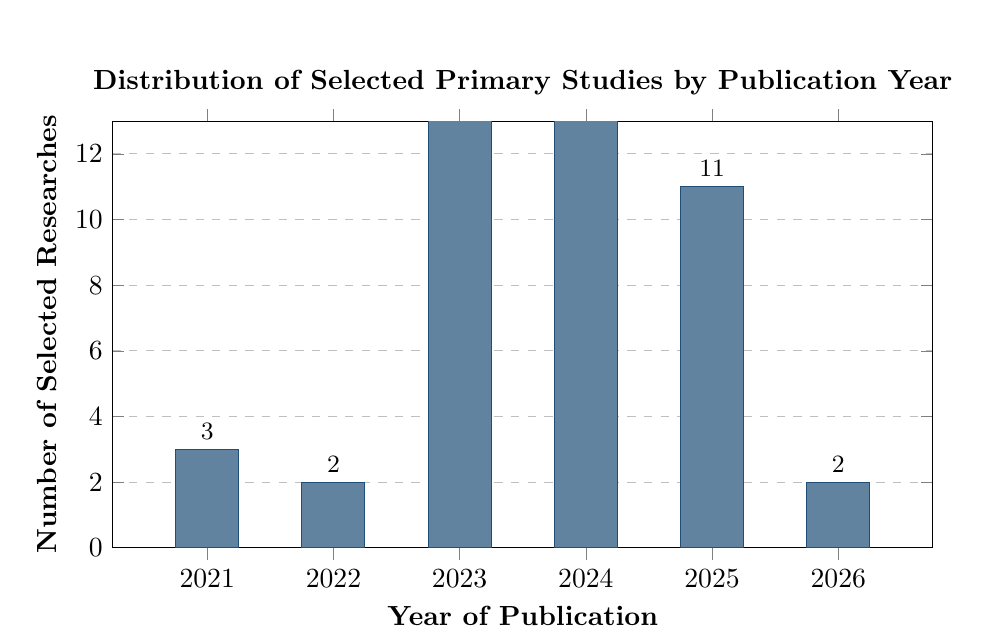
\begin{tikzpicture}
\begin{axis}[
    ybar, width=12cm, height=7cm, bar width=0.8cm,
    ymin=0, ymax=13,
    ylabel={\textbf{Number of Selected Researches}},
    xlabel={\textbf{Year of Publication}},
    symbolic x coords={2021,2022,2023,2024,2025,2026},
    xtick=data, nodes near coords,
    nodes near coords style={font=\small\bfseries},
    ymajorgrids=true, grid style=dashed,
    title={\textbf{Distribution of Selected Primary Studies by Publication Year}},
    enlarge x limits=0.15
]
\addplot[fill=headerblue!70,draw=headerblue] coordinates {
    (2021,3) (2022,2) (2023,14) (2024,14) (2025,11) (2026,2)
};
\end{axis}
\end{tikzpicture}
\caption{Quality assessment showing the temporal distribution of selected primary studies.}
\label{fig:year_distribution}
\end{figure*}

\subsubsection{Data extraction and synthesis}
\label{sec:data_extraction}
Data extraction and synthesis, as shown in Table~\ref{tab:data_extraction}, were performed for each selected research in order to obtain the answers to the research questions. The ten attributes cover both bibliographic extraction and analytical synthesis.

\begin{table*}[!t]
\centering
\caption{Data extraction and synthesis attributes for each selected research.}
\label{tab:data_extraction}
\small
\begin{tabular}{@{}cp{4cm}p{9cm}@{}}
\toprule
\textbf{\#} & \textbf{Attribute} & \textbf{Description} \\
\midrule
\multicolumn{3}{l}{\textit{Extraction of Data}} \\
\midrule
1 & Bibliographic information & Title, author(s), publication year, publisher details, and type (journal/conference/preprint) \\
2 & Overview & The basic proposal and objective of the selected research \\
3 & Results & Quantitative and qualitative results obtained \\
4 & Data collection & Nature of data used (synthetic, benchmark, real-world repositories) \\
5 & Assumptions & Assumptions (if any) required to validate results, including oracle assumptions (e.g., availability of ground-truth test suites at inference time) \\
6 & Validation & Validation method used (benchmark, case study, human evaluation, ablation) \\
\midrule
\multicolumn{3}{l}{\textit{Synthesis of Data}} \\
\midrule
7 & Classification & Relevance to one of the six predefined categories \\
8 & Techniques utilized & Prompting, fine-tuning, RL, retrieval, planning, static analysis, etc. \\
9 & Verification/Repair mechanism & Feedback source, verification signal, iteration budget, and repair strategy (self-critique, taxonomy-guided, CDCL backtracking, ranking, etc.) \\
10 & Tools/Benchmarks identification & Tools, frameworks, and benchmarks used \\
\midrule
\multicolumn{3}{l}{\textit{Extracted synthesis record: Tambon et al.~\cite{tambon2025}}} \\
\midrule
7 & Classification & Bug Detection \& Classification \\
8 & Techniques utilized & Empirical analysis, open coding, stratified sampling, practitioner survey \\
9 & Verification/Repair mechanism & None (observational study; no repair mechanism) \\
10 & Tools/Benchmarks identification & CoderEval \\
\midrule
\multicolumn{3}{l}{\textit{Extracted synthesis record: Wang et al.~\cite{wang2025where}}} \\
\midrule
7 & Classification & Bug Detection \& Classification \\
8 & Techniques utilized & Open coding, thematic analysis, Jaccard similarity, Levenshtein-distance repair-effort analysis \\
9 & Verification/Repair mechanism & None (observational taxonomy study; no automated repair mechanism) \\
10 & Tools/Benchmarks identification & HumanEval \\
\bottomrule
\end{tabular}
\end{table*}

%====================================================================
% SECTION 3 — RESULTS  (mirrors Rashid et al. Section 3)
%====================================================================
\section{Results}
\label{sec:results}
46 primary studies were identified and classified across the six categories. The results are presented through structured synthesis tables, following the methodological guidelines that favor quantitative classification over paragraph-based summaries.

\subsection{Classification of Selected Researches}
\label{sec:classification}
Table~\ref{tab:classification} summarizes the classification of the 46 selected researches into the six predefined categories.

\begin{table*}[!t]
\centering
\caption{Classification of 46 selected researches across the six predefined categories.}
\label{tab:classification}
\small
\begin{tabular}{@{}clcp{7.5cm}@{}}
\toprule
\textbf{\#} & \textbf{Category} & \textbf{Count} & \textbf{Research Identification} \\
\midrule
1 & General & 8 & Dou et al.~\cite{dou2026}, Ding et al.~\cite{ding2025codingcare} (CodingCare), Xia et al.~\cite{xia2025agentless} (Agentless), Jin et al.~\cite{jin2023inferfix} (InferFix), Zhang et al.~\cite{zhang2024autocoderover} (AutoCodeRover), Jimenez et al.~\cite{jimenez2024swebench} (SWE-bench), Le et al.~\cite{le2022coderl} (CodeRL), Jain et al.~\cite{jain2024} (LiveCodeBench) \\
\midrule
2 & Code Generation & 8 & Li et al.~\cite{li2025scot} (SCoT), Jiang et al.~\cite{jiang2024selfplan} (Self-Planning), Chen et al.~\cite{chen2021humaneval} (HumanEval), Austin et al.~\cite{austin2021mbpp} (MBPP), Hendrycks et al.~\cite{hendrycks2021apps} (APPS), Zhang et al.~\cite{zhang2025abfcg} (ABFCG), Li et al.~\cite{li2024deveval} (DevEval), Du et al.~\cite{du2023classeval} (ClassEval) \\
\midrule
3 & Bug Detection \& Classification & 4 & Dou et al.~\cite{dou2026}*, Tambon et al.~\cite{tambon2025}, Wang et al.~\cite{wang2025where}, Pan et al.~\cite{pan2024lost} \\
\midrule
4 & Verification \& Test Generation & 10 & Liu et al.~\cite{liu2025llm4tdg} (LLM4TDG), Chen et al.~\cite{chenbei2023} (CodeT), Ni et al.~\cite{ni2023lever} (LEVER), Ma et al.~\cite{ma2025saga} (SAGA), Sun et al.~\cite{sun2024clover} (Clover), Zhong et al.~\cite{zhong2024ldb} (LDB)*, Liu et al.~\cite{liu2023evalplus} (EvalPlus), Zhang et al.~\cite{zhangt2023coderreviewer} (Coder-Reviewer reranking), Lemieux et al.~\cite{lemieux2023codamosa}, Zhang et al.~\cite{zhang2023algo} (ALGO) \\
\midrule
5 & Iterative Self-Repair & 10 & Xia et al.~\cite{xia2023apr}, Chen et al.~\cite{chen2023selfdebug} (Self-Debug), Wang et al.~\cite{wang2024intervenor} (INTERVENOR), Olausson et al.~\cite{olausson2024}, Madaan et al.~\cite{madaan2023} (Self-Refine), Shinn et al.~\cite{shinn2023} (Reflexion), Zhong et al.~\cite{zhong2024ldb} (LDB)*, Zhang et al.~\cite{zhang2023selfedit} (Self-Edit), Xia \& Zhang~\cite{xia2024chatrepair} (ChatRepair), Ding et al.~\cite{ding2024cycle} (CYCLE) \\
\midrule
6 & Optimization \& Security & 9 & Zhao et al.~\cite{zhao2025semopt} (SemOpt), Jonnala et al.~\cite{jonnala2025}, Lyu et al.~\cite{lyu2025toppass} (Top Pass), Zhang et al.~\cite{zhang2024copilot} (Copilot-in-the-Loop), Bruni et al.~\cite{bruni2025}, Nazzal et al.~\cite{nazzal2024promsec} (PromSec), Ding et al.~\cite{ding2025codingcare}*, Pearce et al.~\cite{pearce2022}, He \& Vechev~\cite{he2023sven} (SVEN) \\
\midrule
\multicolumn{2}{r}{\textbf{Total category assignments:}} & 49 & \\
\multicolumn{2}{r}{\textbf{Total distinct studies:}} & 46 & \\
\bottomrule
\end{tabular}
\begin{flushleft}
\footnotesize * indicates studies appearing in multiple categories due to their multi-faceted contributions.
\end{flushleft}
\end{table*}

Within the General category, Dou et al.~\cite{dou2026} integrate bug characterization with repair evaluation, while Ding et al.'s CodingCare~\cite{ding2025codingcare} spans generation and security assurance. Xia et al.'s Agentless~\cite{xia2025agentless} provides a disciplined single-agent pipeline for repository-level issue resolution, combining hierarchical fault localization, search/replace patch generation, and regression-plus-reproduction-test validation, achieving 32.00\% on SWE-bench Lite at \$0.70 per issue.

Jin et al.'s InferFix~\cite{jin2023inferfix} offers a complementary industrial perspective on the end-to-end pipeline: the Infer static analyzer detects, classifies, and localizes bugs (null dereference, resource leak, thread safety violation); a dense retriever then fetches semantically similar historic fixes; and a finetuned 12B Codex model generates patches guided by bug-type annotations, localization markers, and extended syntactic context (eWASH). Achieving 76.8\% top-1 repair accuracy in Java and 65.6\% in C\#, InferFix demonstrates that \textit{taxonomy-aware, retrieval-augmented} single-shot repair can outperform generic few-shot and instruction-based LLM baselines by 8.6--13\% absolute. It is deployed as a GitHub Action within Microsoft's CI pipeline, validating patches through build, regression test, and re-analysis stages.

Zhang et al.~\cite{zhang2024autocoderover} present AutoCodeRover, a single-agent autonomous program improvement system that operates directly on repository-level issue reports without multi-agent orchestration. It employs a two-stage pipeline: (1) a context retrieval agent navigates the project AST via structured APIs (search\_class, search\_method, etc.) using a stratified search strategy of up to ten iterations, and (2) a patch generation agent crafts patches with a format-constrained retry loop (up to three attempts) validated by a linter and optionally by test execution. On SWE-bench Lite, AutoCodeRover resolves 19\% of issues at pass@1 (37k tokens, \$0.43 per issue) and 26\% at pass@3, outperforming the multi-agent Swe-agent baseline (18\%, 245k tokens, \$2.51) at roughly one-sixth the cost. Its challenge taxonomy reveals that even when localization is correct (55.3\% of cases combined success and wrong-patch), patch content errors remain the dominant failure mode (29.3\% wrong patch), underscoring that precise context retrieval alone does not guarantee correct repair---a finding that reinforces the need for taxonomy-guided feedback in the repair loop.

CodeRL~\cite{le2022coderl} is classified as General because it spans code generation, execution-based verification, and critic-guided repair. SWE-bench~\cite{jimenez2024swebench} is a repair-focused repository benchmark, while LiveCodeBench~\cite{jain2024} evaluates generation, self-repair, execution, and test prediction; under the benchmark category-fit rule, both therefore belong to General rather than Code Generation.

Li et al.~\cite{li2024deveval} challenge the ecological validity of function-level benchmarks through DevEval, a manually annotated repository-level code generation benchmark comprising 1,825 samples from 115 real-world Python repositories. Unlike HumanEval and MBPP, where 100\% of samples are standalone functions, DevEval mirrors real-world distributions: 27\% standalone and 73\% non-standalone functions with intra-class, intra-file, and cross-file dependencies. Evaluation of eight LLMs reveals dramatic performance drops: GPT-4's Pass@1 falls from 80\% on HumanEval to 53\% on DevEval (local-file infilling), with Recall@1 for cross-file dependencies as low as 43.8\%. These findings provide empirical grounding for Gap 5 by demonstrating that existing benchmarks systematically overestimate real-world code generation capability.

Du et al.~\cite{du2023classeval} complement the repository-level perspective of DevEval with a focused class-level benchmark, ClassEval, comprising 100 manually constructed Python classes (412 methods) designed to evaluate compositional code generation. Unlike function-level benchmarks where 95.8\% of HumanEval tasks are standalone, ClassEval deliberately structures 76.2\% of its methods with intra-class dependencies (field 65.5\%, method 26.0\%). Evaluation of 11 LLMs reveals catastrophic performance drops: GPT-4's class-level Pass@1 falls to 37.0\% (from 85.4\% on HumanEval), and GPT-3.5 falls to 27.0\% (from 68.9\%). A critical methodological finding is that generation strategy must be model-dependent: holistic generation (entire class at once) is optimal only for GPT-4 and GPT-3.5, whereas incremental or compositional method-by-method generation is superior for all other models, suggesting that long-context comprehension is a bottleneck for non-GPT architectures. Furthermore, field-accessing code is generated correctly far more often than method-invoking code (DEP(F) $\gg$ DEP(M)), indicating that LLMs struggle with dynamic call-graph reasoning even when the class context is fully provided.

Within the Bug Detection \& Classification category, the four retained taxonomic studies provide complementary perspectives. Dou et al.~\cite{dou2026} develop a repair-oriented three-tier/ten-category transformation taxonomy, while Tambon et al.~\cite{tambon2025} derive a practitioner-validated taxonomy of ten bug patterns from real-world CoderEval tasks. Wang et al.~\cite{wang2025where} complement these taxonomies with a two-dimensional empirical characterization of 558 incorrect code snippets generated by six LLMs on the HumanEval benchmark. Through open coding and thematic analysis (Fleiss' $\kappa=0.84$ for semantic characteristics), they identify 13 semantic and 14 syntactic error types. Their analysis reveals that over 40\% of LLM-generated faults manifest as block-level errors (missing or incorrect code blocks) rather than single-token mistakes, and that 84.89\% of incorrect snippets deviate from ground truth by more than 50 Levenshtein edits. Crucially, they demonstrate that different LLMs produce distinct error distributions for the same task, implying that model-agnostic repair strategies may be suboptimal.

Pan et al.~\cite{pan2024lost} extend taxonomic coverage to the code-translation domain, manually analyzing 1,748 bugs across 6,197 translation attempts among five programming languages (C, C++, Go, Java, Python) and seven LLMs. Their taxonomy comprises 15 categories organized into five groups: syntactic and semantic differences between languages (30.5\%), dependency and logic bugs (24.2\%), data-related bugs (33.5\%), model-specific constraints (6.6\%), and others. Notably, they demonstrate that translation bugs differ structurally from generation bugs---for example, 33.5\% of translation bugs are data-related (incorrect data types, input parsing, output formatting), whereas generation taxonomies emphasize block-level logic errors. They further show that iterative prompt crafting with execution-feedback context can improve GPT-4 translation success by 12.33\% in one iteration, with diminishing returns thereafter.

Lemieux et al.~\cite{lemieux2023codamosa} advance the \textit{Verification \& Test Generation} category through a hybrid paradigm that couples search-based software testing (SBST) with LLM test generation. Built atop the Pynguin MOSA implementation, CODAMOSA monitors coverage progress and invokes OpenAI Codex to generate seed test cases when evolutionary search stalls for more than 25 iterations. A novel deserialization pipeline---incorporating partial parsing, callable expansion, and uninterpreted statements for arbitrary syntactic constructs---integrates Codex outputs into SBST's mutable test case representation. On 486 Python modules from 27 projects, CODAMOSA achieves statistically significantly higher coverage than MOSA on 173 benchmarks (average +10 percentage points) and than a Codex-only baseline on 279 benchmarks (average +9 percentage points), despite spending only half the search time of a union baseline. The study demonstrates that LLMs are most effective in SBST not as replacements but as strategic hint providers during coverage plateaus, and that high-temperature sampling (0.8) consistently outperforms greedy decoding for this task.

Zhang et al.~\cite{zhang2023algo} advance the verification dimension through ALGO, a framework that generates reference oracles---semantically correct but inefficient brute-force solutions---via LLM prompting, then uses these oracles to verify and iteratively refine efficient candidate programs. On 165 CodeContests problems and 35 post-GPT-4 LeetCode problems, ALGO achieves 88.5\% oracle correctness on LeetCode and 72\% on CodeContests, with 75\% verdict agreement against the system judge. By substituting LLM-generated oracles for ground-truth test suites, ALGO improves Codex pass@1 by 8$\times$ (0.70\% to 5.60\%) and CodeT by 2.6$\times$ (2.10\% to 5.60\%). The study demonstrates that brute-force oracle generation is significantly easier for LLMs than efficient solution generation (88.5\% vs.\ 41.2\% success rate on LeetCode), and that oracle-derived test cases achieve 94.78\% agreement with the system judge on CodeContests versus 57.39\% for public example cases alone. ALGO therefore occupies a unique position on the verification spectrum: it does not assume hidden ground-truth tests, nor does it rely on the model's parametric knowledge as a judge; instead, it generates an executable specification via exhaustive search and uses execution comparison as the verification signal.

\subsection{Prompting and Reasoning Techniques Utilization}
\label{sec:prompting_results}
Table~\ref{tab:prompting_techniques} summarizes the utilization of prompting and reasoning techniques across the selected researches.

% Counts reconciled against the current 46-study primary set.
\begin{table*}[!t]
\centering
\caption{Prompting and reasoning techniques utilized in selected researches.}
\label{tab:prompting_techniques}
\small
\begin{tabular}{@{}clcp{7cm}@{}}
\toprule
\textbf{\#} & \textbf{Technique} & \textbf{Count} & \textbf{Relevant Researches} \\
\midrule
1 & Zero-shot prompting & 17 & \cite{chen2021humaneval,xia2023apr,wang2024intervenor,shinn2023,sun2024clover,chenbei2023,jimenez2024swebench,jain2024,li2024deveval,du2023classeval,xia2025agentless,zhang2024autocoderover,ni2023lever,zhangt2023coderreviewer,lemieux2023codamosa,zhang2023algo,dou2026} \\
2 & Few-shot prompting & 10 & \cite{austin2021mbpp,hendrycks2021apps,li2025scot,jiang2024selfplan,chen2023selfdebug,xia2023apr,madaan2023,xia2024chatrepair,zhang2025abfcg,jin2023inferfix} \\
3 & Chain-of-Thought (CoT) & 8 & \cite{li2025scot,jonnala2025,bruni2025,ding2025codingcare,chen2023selfdebug,shinn2023,dou2026,olausson2024} \\
4 & Structured Chain-of-Thought (SCoT) & 1 & \cite{li2025scot} \\
5 & Self-Planning & 1 & \cite{jiang2024selfplan} \\
6 & Recursive Criticism \& Improvement (RCI) & 3 & \cite{bruni2025,ding2025codingcare,dou2026} \\
7 & Retrieval-augmented prompting & 2 & \cite{zhang2025abfcg,jin2023inferfix} \\
8 & Self-critique prompting & 7 & \cite{dou2026,chen2023selfdebug,madaan2023,shinn2023,zhang2023selfedit,ding2024cycle,olausson2024} \\
9 & Structured-output debugging prompts & 1 & \cite{zhong2024ldb} (JSON verdict schema / bracketed debug tags) \\
\bottomrule
\end{tabular}
\end{table*}

From Table~\ref{tab:prompting_techniques}, zero-shot prompting is the most frequently utilized technique, appearing in 17 of 46 (37.0\%) selected studies. Overall, 12 of 46 studies (26.1\%) employ at least one form of explicit reasoning scaffolding across CoT, SCoT, Self-Planning, RCI, and self-critique.

\subsection{Verification and Self-Repair Mechanisms Utilization}
\label{sec:repair_results}
Table~\ref{tab:repair_approaches} summarizes the verification and self-repair mechanisms utilized across the selected researches, together with the iteration budget employed by each mechanism family. The iteration budget column is central to RQ3: it records whether repair proceeds for a fixed small number of iterations, a larger fixed bound, or an unbounded/convergence-based schedule.

% Counts reconciled against the current 46-study primary set.
\begin{table*}[!t]
\centering
\caption{Verification and self-repair mechanisms in selected researches, with iteration budgets.}
\label{tab:repair_approaches}
\scriptsize
\resizebox{\textwidth}{!}{%
\begin{tabular}{@{}clccp{5.2cm}@{}}
\toprule
\textbf{\#} & \textbf{Mechanism} & \textbf{Count} & \textbf{Iteration Budget} & \textbf{Relevant Researches} \\
\midrule
1 & Self-critique with compiler/execution feedback & 9 & \makecell[l]{Varied: 2 (Dou et al.); 3 conversation turns (ChatRepair);\\max 4 refinement steps (CYCLE); 1--2 (Self-Edit);\\unbounded/varied (Olausson et al.); 1 repair round (CodeRL);\\patch retry loop up to 3 attempts (AutoCodeRover)} & \cite{dou2026,chen2023selfdebug,wang2024intervenor,olausson2024,zhang2023selfedit,xia2024chatrepair,ding2024cycle,le2022coderl,zhang2024autocoderover} \\
2 & \makecell[l]{Pure self-critique\\(no execution feedback)} & 1 & \makecell{Task-specific (3--5,\\no fixed cross-activity budget)} & \cite{madaan2023} \\
3 & Bug-taxonomy-guided repair & 2 & 2 (Dou et al.); single-shot / N/A (InferFix) & \cite{dou2026,jin2023inferfix} \\
4 & LLM-generated test verification & 4 & \makecell{CodeT: N/A (post-hoc, no iteration);\\Reflexion trial cap not stated\\(episodic memory: 1 experience for programming)} & \cite{liu2025llm4tdg,shinn2023,ma2025saga,chenbei2023} \\
5 & Runtime-trace / block-level debugging & 1 & \makecell{10 maximum; 20 in robustness check} & \cite{zhong2024ldb} \\
6 & Learned verifier / execution-aware ranking & 2 & N/A (post-hoc) & \cite{ni2023lever,zhangt2023coderreviewer} \\
7 & Static analysis integration (CodeQL/Semgrep/Bandit) & 5 & N/A / pipeline-specific & \cite{bruni2025,ding2025codingcare,nazzal2024promsec,zhao2025semopt,jin2023inferfix} \\
8 & Constraint-based reasoning (CDG/CDCL) & 1 & Iterative constraint repair & \cite{liu2025llm4tdg} \\
9 & Massive-sample generation with entropy/test-based ranking & 3 & N/A (post-hoc) & \cite{xia2023apr,lyu2025toppass,chenbei2023} \\
10 & Benchmark test-adequacy hardening & 2 & N/A & \cite{liu2023evalplus,ma2025saga} \\
11 & \makecell[l]{Formal-specification consistency checking\\(deductive verification + LLM reconstruction)} & 1 & \makecell{$k=1$/$k=10$ independent resampling\\(not feedback-conditioned)} & \cite{sun2024clover}\ (Clover) \\
12 & Critical analysis of the self-repair paradigm & 1 & varied & \cite{olausson2024} \\
13 & LLM-generated oracle verification (brute-force reference) & 1 & Iterative coder refinement on oracle-comparison failures & \cite{zhang2023algo} \\
14 & Coverage-guided LLM-assisted test generation (SBST hybrid) & 1 & Seeds injected when SBST coverage plateaus $>$25 iterations & \cite{lemieux2023codamosa} \\
\bottomrule
\end{tabular}
}
\end{table*}

Self-critique with compiler or execution feedback is the most frequently represented mechanism, appearing in 9 of 46 studies (19.6\%). Among the constraint-based approaches, \cite{liu2025llm4tdg} stands out by combining a constraint dependency graph with conflict-driven clause learning (CDCL) to iteratively repair syntactic and semantic errors in test drivers. Their framework achieves a 47.62\% constraint understanding gain and raises the average \texttt{pass@k} of nine LLMs by 10.41\% (up to 18.66\% for CodeQwen-chat) on HUMANEVAL and HUMANEVAL+. It further demonstrates effectiveness on real-world security testing tasks, detecting malicious behavior in compromised PyPI dependency libraries by generating correct, executable test cases.

\subsection{Preliminary Tools Identification}
\label{sec:tools_prelim}
Once the researches are classified into different categories, the next step is to identify the tools and frameworks used in the selected researches to perform the various activities. Table~\ref{tab:tools_prelim} presents the preliminary identification, grouped by primary activity.

\begin{table*}[p]
\centering
\caption{Preliminary identification of 39 tools and frameworks in selected researches.}
\label{tab:tools_prelim}
\small
\begin{tabular}{@{}clp{7.5cm}@{}}
\toprule
\textbf{\#} & \textbf{Tool/Framework} & \textbf{Relevant Researches} \\
\midrule
\multicolumn{3}{l}{\textit{Generation Approaches (3)}} \\
\midrule
1 & SCoT~\cite{li2025scot} & \cite{li2025scot} \\
2 & Self-Planning~\cite{jiang2024selfplan} & \cite{jiang2024selfplan} \\
3 & ABFCG~\cite{zhang2025abfcg} & \cite{zhang2025abfcg} \\
\midrule
\multicolumn{3}{l}{\textit{General / Cross-Activity Tools (1)}} \\
\midrule
4 & CodeRL~\cite{le2022coderl} & \cite{le2022coderl} \\
\midrule
\multicolumn{3}{l}{\textit{Verification \& Test Generation Tools (9)}} \\
\midrule
5 & LLM4TDG~\cite{liu2025llm4tdg} & \cite{liu2025llm4tdg} \\
6 & Clover~\cite{sun2024clover} & \cite{sun2024clover} \\
7 & CodeT~\cite{chenbei2023} & \cite{chenbei2023} \\
8 & EvalPlus~\cite{liu2023evalplus} & \cite{liu2023evalplus} \\
9 & Coder-Reviewer reranking~\cite{zhangt2023coderreviewer} & \cite{zhangt2023coderreviewer} \\
10 & LEVER~\cite{ni2023lever} & \cite{ni2023lever} \\
11 & SAGA / TCGBench~\cite{ma2025saga} & \cite{ma2025saga} \\
12 & CODAMOSA~\cite{lemieux2023codamosa} & \cite{lemieux2023codamosa} \\
13 & ALGO~\cite{zhang2023algo} & \cite{zhang2023algo} \\
\midrule
\multicolumn{3}{l}{\textit{Iterative Self-Repair Tools (14)}} \\
\midrule
14 & Self-Debug~\cite{chen2023selfdebug} & \cite{chen2023selfdebug,dou2026} \\
15 & INTERVENOR~\cite{wang2024intervenor} & \cite{wang2024intervenor,dou2026} \\
16 & Dou et al.\ repair pipeline~\cite{dou2026} & \cite{dou2026} \\
17 & Xia et al.~\cite{xia2023apr} & \cite{xia2023apr} \\
18 & Self-Refine~\cite{madaan2023} & \cite{madaan2023} \\
19 & Reflexion~\cite{shinn2023} & \cite{shinn2023} \\
20 & Self-Edit~\cite{zhang2023selfedit} & \cite{zhang2023selfedit} \\
21 & ChatRepair~\cite{xia2024chatrepair} & \cite{xia2024chatrepair} \\
22 & CYCLE~\cite{ding2024cycle} & \cite{ding2024cycle} \\
23 & Olausson et al.\ self-repair study~\cite{olausson2024} & \cite{olausson2024} \\
24 & LDB~\cite{zhong2024ldb} & \cite{zhong2024ldb} \\
25 & Agentless~\cite{xia2025agentless} & \cite{xia2025agentless} \\
26 & InferFix~\cite{jin2023inferfix} & \cite{jin2023inferfix} \\
27 & AutoCodeRover~\cite{zhang2024autocoderover} & \cite{zhang2024autocoderover} \\
\midrule
\multicolumn{3}{l}{\textit{Static Analysis Tools (3)}} \\
\midrule
28 & CodeQL & \cite{bruni2025,ding2025codingcare} \\
29 & Semgrep & \cite{bruni2025,zhao2025semopt} \\
30 & Bandit & \cite{ding2025codingcare,nazzal2024promsec} \\
\midrule
\multicolumn{3}{l}{\textit{Optimization \& Security Tools (9)}} \\
\midrule
31 & Jonnala et al.~\cite{jonnala2025} & \cite{jonnala2025} \\
32 & Bruni et al.~\cite{bruni2025} & \cite{bruni2025} \\
33 & SemOpt~\cite{zhao2025semopt} & \cite{zhao2025semopt} \\
34 & Top Pass~\cite{lyu2025toppass} & \cite{lyu2025toppass} \\
35 & Copilot-in-the-Loop~\cite{zhang2024copilot} & \cite{zhang2024copilot} \\
36 & PromSec~\cite{nazzal2024promsec} & \cite{nazzal2024promsec} \\
37 & CodingCare~\cite{ding2025codingcare} & \cite{ding2025codingcare} \\
38 & SVEN~\cite{he2023sven} & \cite{he2023sven} \\
39 & Pearce et al.~\cite{pearce2022} & \cite{pearce2022} \\
\bottomrule
\end{tabular}
\end{table*}

\subsection{Overview of Selected Researches}
\label{sec:overview_researches}
We extract the important data for each selected research according to the attributes defined in Table~\ref{tab:data_extraction} in order to obtain the answers to our research questions. Due to length constraints, the complete extraction sheet for each study is maintained separately and summarized through the synthesis tables of this section.
% NOTE: keep one extraction sheet per paper (10 attributes of Table 2).

%====================================================================
% SECTION 4 — TOOLS AND BENCHMARKS INVESTIGATION (mirrors Rashid Sec. 4)
%====================================================================
\section{Tools and Benchmarks Investigation}
\label{sec:tools_investigation}
On the basis of the SLR, 39 preliminary tools have been identified as given in Table~\ref{tab:tools_prelim}. However, the identification of the given tools is not sufficient to facilitate researchers and practitioners in particular tool selection. Therefore, we further evaluate the selected tools to provide a rational representation. First, an initial evaluation is performed, and then various important characteristics of the tools are used for evaluation.

\subsection{Initial Tools Evaluation}
\label{sec:initial_eval}
In this phase, we perform an initial evaluation of the selected tools (Table~\ref{tab:tools_prelim}) to check the availability of sufficient information required for detailed evaluation. This includes artifact availability, license type, supported models, and documentation. Furthermore, we also search for important tools frequently used in research and industrial practice that may have been missed during the SLR. Tools lacking adequate public information are excluded from further evaluation.

\subsection{Tools Characteristics}
\label{sec:char_defined}
Two types of tools characteristics are used in this article: general characteristics and activity-specific characteristics.

\subsubsection{General characteristics}
These characteristics are applicable to all the tools:
\begin{itemize}[leftmargin=*]
\item \textbf{License type:} Open-source (MIT, Apache-2.0, GPL, MPL) or proprietary; artifact availability is recorded where no formal license is stated.
\item \textbf{Customizability:} ``Full'' (source code modifiable), ``Partial'' (configuration/extension supported), ``No'' (closed).
\item \textbf{Supported LLMs:} Models with which the tool has been demonstrated (e.g., GPT-3.5/4, DeepSeek, CodeLlama).
\item \textbf{Languages:} Programming languages covered by the tool's evaluation.
\end{itemize}

\subsubsection{Activity-specific characteristics}
\begin{itemize}[leftmargin=*]
\item \textbf{Generation approaches:} Supported prompting strategy (CoT/SCoT/Self-Planning), planning support, verification-in-the-loop.
\item \textbf{Verification tools:} Verification signal (compiler / ground-truth tests / generated tests / runtime traces / learned verifier), oracle assumption (whether ground-truth tests are assumed available at inference time), cost per candidate.
\item \textbf{Repair tools:} Feedback source (compiler / unit tests / static analysis / critique), iteration budget, taxonomy use.
\item \textbf{Optimization tools:} Optimization dimension (correctness / efficiency / readability), algorithm type.
\item \textbf{Security tools:} CWE coverage, detection method (static / dynamic / hybrid).
\end{itemize}

\subsection{Tools Evaluation Outcomes}
\label{sec:comparison}

\subsubsection{Comparison of general-category approaches}
\begin{table*}[!t]
\centering
\caption{Comparison of general-category approaches.}
\label{tab:cmp_general}
\footnotesize
\setlength{\tabcolsep}{2.8pt}
\renewcommand{\arraystretch}{1.1}
\begin{tabularx}{\textwidth}{@{}p{58pt}p{58pt}p{38pt}p{72pt}p{58pt}p{75pt}p{42pt}X@{}}
\toprule
\multirow{2}{*}{\textbf{Tool Name}} & \multicolumn{4}{c}{\textbf{General Characteristics}} & \multicolumn{3}{c}{\textbf{Activity-Specific Characteristics}} \\
\cmidrule(lr){2-5} \cmidrule(lr){6-8}
 & \textbf{License} & \textbf{Custom.} & \textbf{Supported LLMs} & \textbf{Languages} & \textbf{Prompting Strategy} & \textbf{Planning} & \textbf{Verification-in-Loop} \\
\midrule
CodeRL~\cite{le2022coderl} & BSD-3-Clause (Salesforce GitHub) & Full & CodeT5-large (770M, primary); GPT-J, GPT-Neo (ablation) & Python & RL fine-tuning + critic-based repair & Yes & Yes (max 1 repair+refine round) \\
\bottomrule
\end{tabularx}
\end{table*}

\subsubsection{Comparison of code generation approaches}
\begin{table*}[!t]
\centering
\caption{Comparison of code generation approaches.}
\label{tab:cmp_generation}
\footnotesize
\setlength{\tabcolsep}{2.8pt}
\renewcommand{\arraystretch}{1.1}
\begin{tabularx}{\textwidth}{@{}p{58pt}p{58pt}p{38pt}p{72pt}p{58pt}p{75pt}p{42pt}X@{}}
\toprule
\multirow{2}{*}{\textbf{Tool Name}} & \multicolumn{4}{c}{\textbf{General Characteristics}} & \multicolumn{3}{c}{\textbf{Activity-Specific Characteristics}} \\
\cmidrule(lr){2-5} \cmidrule(lr){6-8}
 & \textbf{License} & \textbf{Custom.} & \textbf{Supported LLMs} & \textbf{Languages} & \textbf{Prompting Strategy} & \textbf{Planning} & \textbf{Verification-in-Loop} \\
\midrule
SCoT~\cite{li2025scot} & N/A (prompt method) & N/A & Any LLM & Python & Structured CoT & Implicit & No \\
Self-Planning~\cite{jiang2024selfplan} & N/A (prompt method) & N/A & Any LLM & \makecell{Python/Java/\\Go/JavaScript} & Plan-then-generate & Yes & No \\
ABFCG~\cite{zhang2025abfcg} & N/A & Partial & Custom (RetNet) & Java & KG-based retrieval & No & No \\
\bottomrule
\end{tabularx}
\end{table*}

\subsubsection{Comparison of verification and test generation tools}
\begin{table*}[!t]
\centering
\caption{Comparison of verification and test generation tools.}
\label{tab:cmp_verification}
\footnotesize
\setlength{\tabcolsep}{3pt}
\renewcommand{\arraystretch}{1.15}
\begin{tabularx}{\textwidth}{@{}p{48pt}p{55pt}p{30pt}p{68pt}p{62pt}p{72pt}p{78pt}X@{}}
\toprule
\multirow{2}{*}{\textbf{Tool Name}} & \multicolumn{4}{c}{\textbf{General Characteristics}} & \multicolumn{3}{c}{\textbf{Activity-Specific Characteristics}} \\
\cmidrule(lr){2-5} \cmidrule(lr){6-8}
 & \textbf{License} & \textbf{Custom.} & \textbf{Supported LLMs} & \textbf{Languages} & \textbf{Verification Signal} & \textbf{Oracle Assumption} & \textbf{Cost per Candidate} \\
\midrule
LLM4TDG~\cite{liu2025llm4tdg} & N/A & N/A & 9 LLMs & Python & Runtime + CDG constraints & No hidden tests assumed & Not reported \\
CodeT~\cite{chenbei2023} & Code available (\url{github.com/microsoft/CodeT}); no formal license stated & Full & Codex (code-cushman-001, code-davinci-001, code-davinci-002), INCODER-6B, CODEGEN-MONO-16B & Python & LLM-generated input--output tests + candidate execution + dual execution agreement over consensus sets & No ground-truth tests used for selection; hidden benchmark tests used only for final pass@k evaluation & Higher than pure generation---requires both code and test sampling (up to $2\times$ generation calls); tunable down to 10 test samples with modest performance loss \\
EvalPlus~\cite{liu2023evalplus} & Apache License 2.0 & High (open-source; pluggable backends) & Any model via supported inference backends & Python & Augmented test suites & Benchmark-side & N/A \\
Coder-Reviewer reranking~\cite{zhangt2023coderreviewer} & CC BY-NC-SA 4.0 & Full [INFERRED] & Codex-002/001/Cushman; InCoder-6B/1B; CodeGen-16B/6B/2B & Python, SQL, Bash & Coder-reviewer likelihood reranking; optional executability filtering & None for reranking [INFERRED]; execution environment needed for optional filtering & One additional Reviewer likelihood-scoring pass per candidate [INFERRED]; optional execution \\
LEVER~\cite{ni2023lever} & MIT; code/data/checkpoints available & Full & Codex (code-davinci-002), InCoder-6B, CodeGen-16B-multi & SQL (Spider, WikiTQ), Python (GSM8k, MBPP) & Learned verifier + execution & No hidden correctness tests at inference [INFERRED]; execution inputs/context required & One execution + one verifier forward pass per candidate [INFERRED]; verifier $\sim$0.5\% of generator size \\
SAGA / TCGBench~\cite{ma2025saga} & Code/data available (github.com/open-compass/SAGA) & Full & DeepSeek-V3-0324, Qwen2.5-72B-Instruct, Qwen2.5-Coder-32B/7B-Instruct & Python, C++ (evaluated languages for CodeCompass); problems sourced from AtCoder/Codeforces/Nowcoder & LLM-generated tests (Input-Interpreter style) + structured human priors & Requires golden reference solution + human submission corpus (no oracle-free operation) & 1 LLM analysis call per problem (one-time) + $N$ program executions per test case \\
Clover~\cite{sun2024clover} & Code/data available (github.com/ChuyueSun/Clover) & Full & GPT-4 (primary); CodeLlama-34b (ablation, found largely incapable) & Dafny (primary); Verus/Rust (preliminary, 41 examples) & 6-edge consistency check (5 LLM reconstruction/equivalence tests + 1 deductive Dafny/Z3 soundness proof) & No hidden test suite; requires formal (Dafny/Verus) annotations & Not reported \\
LDB~\cite{zhong2024ldb}\footnotemark & Code available (GitHub: FloridSleeves/LLMDebugger) & Full & GPT-3.5, CodeLlama-34B, StarCoder-15B (+GPT-4, GPT-4o backbone ablation) & Python; C++$\to$Python (TransCoder) & Runtime traces (block-level) & Partial (visible test needed to trigger debugging; TransCoder uses all tests as visible, no held-out oracle there) & $\sim$23K tokens/program; 17.23s vs.\ 17.08s for Self-Debugging \\
CODAMOSA~\cite{lemieux2023codamosa} & Open source (GitHub) & Full & Codex (OpenAI API) & Python & Line + branch coverage (SBST fitness) & No hidden tests; coverage-guided only & $\sim$60 Codex queries + 413s API wait per 10-min run \\
ALGO~\cite{zhang2023algo} & Open source (GitHub) & Full & ChatGPT Code Interpreter (verifier); Codex/CodeT/PG-TD/ChatGPT (coder) & Python & LLM-generated brute-force oracle + execution comparison & No hidden tests; oracle is LLM-generated brute-force & One oracle generation + input generator per problem; reusable across coders \\
\bottomrule
\end{tabularx}
\end{table*}
\footnotetext{LDB is counted once in the 39-tool total under Iterative Self-Repair; shown here for its runtime-trace verification signal.}

\subsubsection{Comparison of iterative self-repair tools}
\begin{table*}[!t]
\centering
\caption{Comparison of iterative self-repair tools.}
\label{tab:cmp_repair}
\footnotesize
\setlength{\tabcolsep}{2.5pt}
\renewcommand{\arraystretch}{1.12}
\begin{tabularx}{\textwidth}{@{}p{48pt}p{48pt}p{28pt}p{68pt}p{48pt}p{65pt}p{30pt}p{72pt}X@{}}
\toprule
\multirow{2}{*}{\textbf{Tool Name}} & \multicolumn{4}{c}{\textbf{General Characteristics}} & \multicolumn{4}{c}{\textbf{Activity-Specific Characteristics}} \\
\cmidrule(lr){2-5} \cmidrule(lr){6-9}
 & \textbf{License} & \textbf{Custom.} & \textbf{Supported LLMs} & \textbf{Languages} & \textbf{Feedback Source} & \textbf{Iterative} & \textbf{Iteration Budget} & \textbf{Taxonomy} \\
\midrule
Self-Debug~\cite{chen2023selfdebug} & N/A & N/A & Any LLM & Python/SQL/C++ & Compiler + execution & Yes & Up to 10 rounds (default) & No \\
INTERVENOR~\cite{wang2024intervenor} & Code/data available & Full & GPT-3.5, CodeLlama-7B/13B & Python, C++, Java, JavaScript & Compiler + CoR & Yes & Max 5 conversation turns (Chain-of-Repair) & No \\
Dou et al.~\cite{dou2026} & Artifact available & Partial & 9 LLMs & Python & Compiler + Taxonomy & Yes & 2 & 3 primary / 10 secondary \\
Xia et al.~\cite{xia2023apr} & Code/data available & Full & 9 LLMs (Codex etc.) & Java/Python/C & Test-suite validation (post-hoc) & No & N/A & No \\
Self-Refine~\cite{madaan2023} & Code/data/prompts available & Full & GPT-3.5, ChatGPT, GPT-4, Codex (code-davinci-002) & Python & Self-critique (no execution) & Yes & Task-specific, 3--5 (no fixed budget) & No \\
Reflexion~\cite{shinn2023} & Code/demos/datasets available & Full & GPT-3.5/4, CodeLlama-34B (seed gen.\ via HumanEval-X), starchat-beta (ablation) & Python; Rust (via MultiPL-E) & Self-generated tests + verbal self-reflection (episodic memory) & Yes & Not stated for programming in-paper & No \\
Self-Edit~\cite{zhang2023selfedit} & Code available (dataset not released) & Full & PyCodeGPT-110M, GPT-Neo-125M/1.3B, CodeGen-350M/2B, InCoder-1B, GPT-J-6B, text-davinci-002 (175B) & Python & Execution results (example test case only) & Yes & 1 (2 tested in ablation, mixed/negative on APPS-test) & No \\
ChatRepair~\cite{xia2024chatrepair} & Code available (artifact released with paper) & Full & ChatGPT (gpt-3.5-turbo-0301) & Java, Python & Test execution + compilation errors + conversational history & Yes & Max conversation length 3 (default); up to 200 total queries per bug & No \\
CYCLE~\cite{ding2024cycle} & Code/data/checkpoints available (\url{github.com/ARiSE-Lab/CYCLE_OOPSLA_24}) & Full & CodeGen-350M/2.7B, StarCoder-1B/3B (fine-tuned) & Python & Execution results (test-suite failures, error messages) + past faulty generation & Yes & Max 4 refinement steps (inference default) & No \\
LDB~\cite{zhong2024ldb} & Code available (GitHub: FloridSleeves/LLMDebugger) & Full & GPT-3.5, CodeLlama-34B, StarCoder-15B (+GPT-4, GPT-4o backbone ablation) & Python; C++$\to$Python (TransCoder) & Block-level runtime traces + LLM verdicts & Yes & Max 10 (extends to 20 in ablation: 82.9\%$\to$84.1\%, diminishing returns) & No \\
Olausson et al.~\cite{olausson2024} & Code/data available & Full & CodeLlama-13b-instruct, GPT-3.5, GPT-4 & Python & LLM-generated explanation from execution errors & Yes & Variable (swept as independent variable, $n_p \times n_{fr}$ grid) & No \\
Agentless~\cite{xia2025agentless} & Open-source (MIT) & Full & GPT-4o (primary); GPT-4 (ablation) & Python & Regression + generated reproduction tests & No & N/A (40 candidate patches via 4$\times$10 sampling; majority-vote selection) & No \\
InferFix~\cite{jin2023inferfix} & Proprietary (Microsoft internal) & No & Codex Cushman (12B, finetuned) & Java, C\# & Static analyzer (Infer) + retrieved similar fixes & No & N/A (single-shot retrieval-augmented generation) & Yes (Infer bug-type annotation: NPD/RL/TSV) \\
AutoCodeRover~\cite{zhang2024autocoderover} & Open source (MIT) & Full & GPT-4 (gpt-4-0125-preview) & Python & Test execution + SBFL + linter & Yes (patch retry loop up to 3 attempts) & Context retrieval $\leq$10 strata; patch gen $\leq$3 retries & No \\
\bottomrule
\end{tabularx}
\end{table*}

\subsubsection{Comparison of optimization tools}
\begin{table*}[!t]
\centering
\caption{Comparison of code optimization tools and techniques.}
\label{tab:cmp_optimization}
\footnotesize
\setlength{\tabcolsep}{2pt}
\renewcommand{\arraystretch}{1.1}
\begin{tabularx}{\textwidth}{@{}p{65pt}p{52pt}p{32pt}p{75pt}p{70pt}p{100pt}X@{}}
\toprule
\multirow{2}{*}{\textbf{Tool Name}} & \multicolumn{3}{c}{\textbf{General Characteristics}} & \multicolumn{3}{c}{\textbf{Activity-Specific Characteristics}} \\
\cmidrule(lr){2-4} \cmidrule(lr){5-7}
 & \textbf{License} & \textbf{Custom.} & \textbf{Supported LLMs} & \textbf{Dimension} & \textbf{Algorithm} & \textbf{Languages} \\
\midrule
SemOpt~\cite{zhao2025semopt} & Artifact available & Full & DeepSeek-V3, GPT-4.1, Gemini-2.5 & Efficiency & Rule-based (Semgrep) & C/C++, Python \\
Jonnala et al.~\cite{jonnala2025} & N/A & N/A & GPT-3.5-Turbo, GPT-4-Turbo, GPT-4o-Mini & Time + Memory & CoT + Fine-tuning & Python \\
Top Pass~\cite{lyu2025toppass} & N/A & N/A & ChatGPT, DeepSeek-Coder & Ranking & pass@k loss & Python \\
Copilot-in-the-Loop~\cite{zhang2024copilot} & Proprietary & No & Copilot Chat & Quality/Maintainability (code smells) & Prompt-based (name-specificity) & Python \\
\bottomrule
\end{tabularx}
\end{table*}

\subsubsection{Comparison of security tools}
\begin{table*}[!t]
\centering
\caption{Comparison of security-focused tools in LLM code generation.}
\label{tab:cmp_security}
\footnotesize
\setlength{\tabcolsep}{2pt}
\renewcommand{\arraystretch}{1.1}
\begin{tabularx}{\textwidth}{@{}p{55pt}p{55pt}p{30pt}p{65pt}p{48pt}p{88pt}p{65pt}X@{}}
\toprule
\multirow{2}{*}{\textbf{Tool Name}} & \multicolumn{4}{c}{\textbf{General Characteristics}} & \multicolumn{3}{c}{\textbf{Activity-Specific Characteristics}} \\
\cmidrule(lr){2-5} \cmidrule(lr){6-8}
 & \textbf{License} & \textbf{Custom.} & \textbf{Supported LLMs} & \textbf{Languages} & \textbf{CWE Coverage} & \textbf{Detection} & \textbf{Method} \\
\midrule
PromSec~\cite{nazzal2024promsec} & Demo code available & Partial & GPT-3.5/4, Bard, CodeLlama & Python/Java & High & Bandit + SpotBugs & Static \\
CodingCare~\cite{ding2025codingcare} & N/A & N/A & DeepSeek, Mistral, CodeLlama (7B) & Python & \makecell[l]{6 types: DoS, Code Execution,\\ Buffer Overflow, Memory Corruption,\\ SQL Injection, XSS} & CodeQL + Bandit & Static \\
Bruni et al.~\cite{bruni2025} & GPL-3.0 & Full & GPT-3.5/4o-Mini/4o & Python/C & 18+ CWEs & Semgrep + CodeQL & Static \\
SVEN~\cite{he2023sven} & Code available (eth-sri/sven) & Full & CodeGen-350M/2.7B/6.1B (primary); InCoder, SantaCoder (gen.) & Python, C/C++ & 9 training + 17 transfer (26 eval.) & Training-time (prefix tuning) & Prefix tuning \\
Pearce et al.~\cite{pearce2022} & Dataset available (Zenodo) & N/A & GitHub Copilot (Codex) & Python, C, Verilog & 18 CWEs (MITRE Top 25) & CodeQL + Manual & Empirical study \\
\bottomrule
\end{tabularx}
\begin{flushleft}
\footnotesize \textit{CodingCare result:} $\geq$50\% reduction (up to 100\% on 2 of 5 test projects).
\textit{PromSec result:} reduces total CWE count from 164 (ablation without gGAN) to 4 while holding 0.97 code-graph similarity; needs as few as 2 LLM queries per fix cycle vs.\ 7 for the matched baseline.
\end{flushleft}
\end{table*}

\subsubsection{Comparison of benchmarks}
\begin{table*}[p]
\centering
\caption{Comparison of benchmarks used in LLM code generation research.}
\label{tab:cmp_benchmarks}
\footnotesize
\setlength{\tabcolsep}{3pt}
\renewcommand{\arraystretch}{1.08}
\begin{tabularx}{\textwidth}{@{}p{92pt}p{55pt}p{70pt}p{105pt}X p{62pt}@{}}
\toprule
\textbf{Benchmark} & \textbf{Size} & \textbf{Language} & \textbf{Source} & \textbf{Focus} & \textbf{Leakage Risk} \\
\midrule
HumanEval/HumanEval+~\cite{chen2021humaneval,chenbei2023} & 164 & Python & Hand-crafted / augmented tests & Correctness & High \\
MBPP/MBPP+~\cite{austin2021mbpp,chenbei2023} & \makecell{974 / 399;\\CodeT: 427\\(sanitized subset)} & Python & Crowd-sourced / augmented tests & Correctness & Moderate \\
APPS/APPS+~\cite{hendrycks2021apps,chenbei2023} & 10{,}000 / 600 & Python & Codeforces/Kattis / curated & Correctness & Moderate \\
EffiBench~\cite{huang2024effibench} & 1{,}000 & Python & LeetCode & Efficiency & Moderate \\
LLMSecEval~\cite{bruni2025} & 150 & Python/C & CWE-mapped & Security & Low \\
SecurityEval & 130 & Python & Security-focused prompts & Security & Low \\
CodeContests~\cite{lyu2025toppass,chenbei2023} & 13{,}610 & Python (as used in the cited studies) & AlphaCode competitive programming & Competitive correctness & Unknown \\
SWE-bench~\cite{jimenez2024swebench} & 2{,}294 (Lite: 300) & Python & 12 real GitHub repos, issue+PR pairs & Real-world repair & Low (no pre/post-2023 resolve-rate gap found) \\
RWPB~\cite{dou2026} & 140 & Python & GitHub 2024 & Real-world correctness & Very Low \\
pypi\_malregistry~\cite{liu2025llm4tdg} & 5 packages & Python & Malicious PyPI packages & Security (dynamic testing) & Low \\
Real-world web projects~\cite{ding2025codingcare} & 5 types & Python & Generated web applications & Security & Low \\
SemOpt Benchmark~\cite{zhao2025semopt} & 151 / 150 & C/C++ / Python & GitHub commits & Efficiency/Optimization & Low (exact matches excluded) \\
PromSec dataset~\cite{nazzal2024promsec} & 100 Py + 100 Java (test) & Python/Java & MITRE/CodeQL-doc + AixBench/CodeReval & Security & Low \\
Copilot-in-the-Loop dataset~\cite{zhang2024copilot} & 102 smells (92--93 usable snippets) & Python & 311 GitHub-sourced files & Maintainability/code smells & Unknown \\
HumanEval-X~\cite{wang2024intervenor} & 820 & C++, Java, JavaScript, Go, Python & Multilingual HumanEval translations & Code translation & Unknown \\
TransCoder~\cite{zhong2024ldb} & Not stated in LDB & C++$\rightarrow$Python & TransCoder translation benchmark & Code translation/debugging & Unknown \\
CodeError~\cite{wang2024intervenor} & 4{,}463 & Python & INTERVENOR-constructed erroneous programs & Code repair & Unknown \\
DS-1000~\cite{wang2024intervenor} & 1{,}000 & Python & Data-science coding problems across seven libraries & Data-science correctness & Unknown \\
Defects4J 1.2~\cite{xia2023apr} & 391 (255 single-function) & Java & Real-world open-source projects & Correctness/repair & Unknown \\
Defects4J 2.0~\cite{xia2023apr} & 438 (228 single-function) & Java & Real-world open-source projects & Correctness/repair & Unknown \\
QuixBugs-Java/Python~\cite{xia2023apr} & 40 per language & Java/Python & Programming-challenge programs & Multilingual repair & Unknown \\
ManyBugs~\cite{xia2023apr} & 185 (91 reproducible used) & C & Real-world open-source projects & Correctness/repair & Unknown \\
LeetcodeHardGym~\cite{shinn2023} & 40 & Python (infra.\ supports 19 langs) & Post-Oct-2022 Leetcode Hard problems & Contamination-resistant correctness & Very Low (deliberately post-cutoff) \\
CloverBench~\cite{sun2024clover} & 60 base $\times$ 5 variants (300) & Dafny & Hand-crafted textbook programs & Correctness/consistency & Low \\
MBPP-DFY-50~\cite{sun2024clover} & 50 (33 in-scope) & Dafny & Hand-translated from MBPP & Correctness/consistency & Low \\
LiveCodeBench~\cite{jain2024} & 511 (May'23--May'24) & Python & LeetCode, AtCoder, CodeForces contests & Holistic: generation, self-repair, execution, test prediction & Very Low (time-segmented) \\
CoderEval~\cite{tambon2025} & 230 functions & Python & 43 real-world GitHub projects & Real-world LLM bug characterization & Low \\
ConDefect~\cite{xia2024chatrepair} & 651 (321 Java, 330 Python) & Java, Python & Programming contest bugs after Oct 2021 & Correctness/repair (leakage-free) & Very Low \\
DevEval~\cite{li2024deveval} & 1,825 (115 repos) & Python & 115 real-world PyPI repos (manually annotated by 13 developers) & Repository-level code generation (standalone + non-standalone) & Low (0.36\% Pass@1 diff. seen vs. unseen; new requirements) \\
ClassEval~\cite{du2023classeval} & 100 classes (412 methods) & Python & Manually crafted (500 person-hours) & Class-level code generation (holistic, incremental, compositional) & Low (manual construction, no public code reuse) \\
\bottomrule
\end{tabularx}
\end{table*}

\clearpage

%====================================================================
% SECTION 5 — ANSWERS OF RESEARCH QUESTIONS (mirrors Rashid Sec. 5)
%====================================================================
\section{Answers of Research Questions}
\label{sec:answers}

\subsection*{RQ1: What important researches have been reported from 2021 to 2025?}
\textbf{Answer:} 46 important researches selected from the 2021--2025 search window (including two protocol exceptions formally published in 2026) have been identified as per the selection and rejection criteria (Section~\ref{sec:criteria}). These researches are classified into six corresponding categories. The details are as follows:
\begin{itemize}[leftmargin=*]
\item 8 researches have been identified in the \textit{General} category, including end-to-end autonomous improvement (Zhang et al.~\cite{zhang2024autocoderover}), cross-activity critic-guided generation and repair (CodeRL), and the repair-focused or multi-activity benchmarks SWE-bench and LiveCodeBench.
\item 8 researches have been identified in the \textit{Code Generation} category, with three being foundational single-shot benchmark papers (HumanEval, MBPP, APPS), and two class- and repository-level generation benchmarks (DevEval, ClassEval).
\item 4 researches have been identified in the \textit{Bug Detection \& Classification} category, anchored by the complementary taxonomies of Dou et al.~\cite{dou2026}, Tambon et al.~\cite{tambon2025}, Wang et al.~\cite{wang2025where}, and Pan et al.~\cite{pan2024lost}.
\item 10 researches have been identified in the \textit{Verification \& Test Generation} category, including hybrid SBST--LLM test generation (Lemieux et al.~\cite{lemieux2023codamosa}), post-hoc candidate ranking (CodeT), and LLM-generated oracle verification (Zhang et al.~\cite{zhang2023algo}).
\item 10 researches have been identified in the \textit{Iterative Self-Repair} category.
\item 9 researches have been identified in the \textit{Optimization \& Security} category.
\end{itemize}
The overview, publication year, validation method, and description of each selected technique are summarized in Table~\ref{tab:classification}.

\subsection*{RQ2: Which prompting and reasoning techniques are more frequently utilized?}
\textbf{Answer:} As analyzed in Table~\ref{tab:prompting_techniques}, zero-shot prompting is the most frequently utilized technique, appearing in 17 of 46 studies (37.0\%). CodeT uses zero-shot generation for both candidate programs and generated test cases, with a direct structured instruction for producing assertion-style input--output tests rather than a chain-of-thought or planning scaffold~\cite{chenbei2023}. Overall, 12 of 46 studies (26.1\%) employ at least one form of explicit reasoning scaffolding across CoT, SCoT, Self-Planning, RCI, and self-critique, indicating a strong trend toward structured intermediate reasoning in modern LLM code generation research.

\subsection*{RQ3: Which verification and self-repair mechanisms are more frequently utilized, and with what iteration budgets?}
\textbf{Answer:} As shown in Table~\ref{tab:repair_approaches}, self-critique with compiler or execution feedback is the most frequently represented mechanism (9 studies, 19.6\%). Regarding iteration budgets, the reviewed approaches span fixed small budgets ($\leq$3 iterations), larger or unbounded schedules, and post-hoc mechanisms without iteration. CodeT belongs to the last group: it performs one post-hoc verification-and-ranking pass over independently sampled programs and generated tests, without modifying or repairing any candidate~\cite{chenbei2023}. CODAMOSA~\cite{lemieux2023codamosa} represents a structurally different point on the test-generation spectrum: rather than verifying correctness of independently generated candidates, it uses the LLM to produce seed test inputs that guide an evolutionary search algorithm (MOSA) out of coverage plateaus, demonstrating that LLM-generated tests can be deserialized and mutated within an SBST framework to achieve higher coverage than either SBST or LLM alone. The taxonomy-grounded mechanisms now include both Dou et al.'s two-iteration pipeline~\cite{dou2026}, which achieves a 29.2\% repair success rate on GPT-4, and InferFix's single-shot static-analysis taxonomy~\cite{jin2023inferfix}. Constraint-based reasoning, runtime-trace debugging, LLM-generated oracle verification, and coverage-guided SBST--LLM generation remain specialized directions. These results indicate a diversified verification-and-repair landscape in which the iteration budget is rarely treated as a first-class design variable.

ALGO~\cite{zhang2023algo} represents a third verification paradigm: rather than using the LLM to generate test inputs (CODAMOSA) or to judge correctness directly (LLM-as-judge), it prompts the LLM to generate a \textit{reference oracle}---a brute-force solution that is semantically correct but computationally inefficient---and then derives test cases by executing this oracle against random inputs. Candidate programs are verified by output comparison, and failed cases are fed back for iterative coder refinement. This shifts the oracle assumption from ``ground-truth tests available'' to ``brute-force solution generatable,'' which is shown to hold for 88.5\% of LeetCode and 72\% of CodeContests problems.

ChatRepair~\cite{xia2024chatrepair} demonstrates that conversational repair with detailed test-failure feedback achieves 114 correct fixes on Defects4J 1.2 under a default conversation budget of 3 turns, at an average cost of \$0.42 per bug. It relies on ground-truth test suites and perfect fault localization.

Ding et al.'s CYCLE~\cite{ding2024cycle} continues training code LMs on (problem description, faulty generation, execution feedback) tuples to learn self-refinement end-to-end. With a fixed inference budget of 4 refinement steps, CYCLE-350M achieves 47.9\% relative improvement on HumanEval and 63.5\% on MBPP-S over one-time generation, matching models with 3$\times$ more parameters. A Past Generation Mask (PGM) at 5\% masking ratio prevents copy-pasting faulty code.

\subsection*{RQ4: What are the significant tools, frameworks, and benchmarks?}
\textbf{Answer:} On the basis of the SLR, 39 tools/frameworks and 30 benchmarks have been identified to support LLM-based code generation across the five activity dimensions. After the comparative evaluation in Section~\ref{sec:comparison}, the following key tools are presented by activity:
\begin{itemize}[leftmargin=*]
\item 3 \textbf{generation approaches} are presented to support structured prompting, planning, and retrieval augmentation (SCoT, Self-Planning, ABFCG).
\item 9 \textbf{verification and test generation tools} are presented (LLM4TDG, CodeT, Clover, EvalPlus, Coder-Reviewer reranking, LEVER, SAGA/TCGBench, CODAMOSA, ALGO). CodeT is a post-hoc selector rather than a repair tool: it generates tests, executes sampled candidates, and ranks consensus sets through dual execution agreement~\cite{chenbei2023}. The oracle assumption column of Table~\ref{tab:cmp_verification} is decisive for practical deployment: tools assuming hidden ground-truth tests at inference time cannot be transferred directly to production settings.
\item 14 \textbf{repair tools} are presented (Self-Debug, INTERVENOR, Dou et al., Xia et al., Self-Refine, Reflexion, Self-Edit, ChatRepair, CYCLE, Olausson et al., LDB, Agentless, InferFix, AutoCodeRover). Among these, LLM4TDG notably achieves the highest \texttt{pass@k} improvement (18.66\% on CodeQwen-chat) and validates its approach on real malicious packages.
\item 4 \textbf{optimization tools} are presented (SemOpt, Jonnala et al., Top Pass, Copilot-in-the-Loop).
\item 5 \textbf{security tools} are presented (PromSec, CodingCare, Bruni et al., SVEN, Pearce et al.).
\item Three \textbf{static analysis integration tools} are consistently used across security-focused works (CodeQL, Semgrep, Bandit).
\item 30 \textbf{benchmarks} span correctness and translation, repair, data-science programming, efficiency and optimization, maintainability, security, competitive programming, and real-world leakage-free evaluation (RWPB, SWE-bench~\cite{jimenez2024swebench}, LeetcodeHardGym~\cite{shinn2023}, LiveCodeBench).
\end{itemize}

%====================================================================
% SECTION 6 — DISCUSSION AND LIMITATIONS (mirrors Rashid Sec. 6)
%====================================================================
\section{Discussion and Limitations}
\label{sec:discussion}

\subsection{Discussion on Code Generation Techniques}
It is analyzed that prompting and reasoning scaffolds are the core enablers of LLM-based code generation. The evolution from zero-shot prompting through CoT to SCoT and Self-Planning reveals a systematic trend: \textit{the more structured the intermediate representation, the better the downstream code quality}. Structured variants such as SCoT achieve up to 13.79\% improvement over vanilla CoT on HumanEval \cite{li2025scot}, validating this hypothesis empirically. Moreover, reasoning-specialized models (e.g., DeepSeek-R1) that internalize structured reasoning achieve even higher gains (up to 77.9\% on RWPB~\cite{dou2026}), suggesting that the trajectory of future research lies in combining explicit scaffolding with reasoning-enhanced model architectures.

This generation-repair dependency is further emphasized by Tambon et al.~\cite{tambon2025}, who show that switching from docstring-based to human-labeled prompts significantly shifts the distribution of bug patterns (Fisher-exact $p<0.05$), with human-labeled prompts reducing trivial errors (Syntax Error, Silly Mistake) while increasing semantic misinterpretations---precisely the fault class that is hardest to repair automatically.

\subsection{Discussion on Verification}
Verification is the hinge of the generate--verify--repair pipeline: the quality of every downstream repair action is bounded by the quality of the verification signal that triggers it. The reviewed literature exhibits a spectrum of verification signals of increasing granularity: compiler diagnostics, ground-truth test execution, LLM-generated tests---exemplified by CodeT's candidate execution and consensus-set-based dual execution agreement~\cite{chenbei2023}---block-level runtime traces~\cite{zhong2024ldb}, which decompose programs via control-flow-graph analysis and outperform coarser line-level and function-level decompositions on both accuracy and token cost (82.9\% vs.\ 80.5\%/79.9\% on HumanEval with GPT-3.5, at lower token cost), and learned verifiers---Ni et al.'s LEVER reranks sampled candidates using a lightweight classifier (T5/RoBERTa, roughly 0.5\% of the generator's parameter count) trained to predict correctness from the natural-language input, candidate program, and its execution result, requiring no hidden ground-truth tests at inference time~\cite{ni2023lever}. CodeT performs no iteration or repair: it is a single-shot generate-many-then-select method, structurally distinct from every study in the Iterative Self-Repair category. Ma et al.'s SAGA takes the opposite oracle stance from LEVER: it achieves higher detection rates and verifier accuracy than existing TCG baselines by combining LLM reasoning with structured human priors from both correct and incorrect submissions, but explicitly depends on a golden reference solution as interpreter, restricting its direct applicability outside domains where such oracles exist~\cite{ma2025saga}. A decisive practical distinction is the \textit{oracle assumption}: several works implicitly assume the availability of hidden ground-truth test suites at inference time, an assumption that does not hold in production deployment; self-generated verification signals relax this assumption but remain benchmark-dependent in quality. CodeT's test-case toxicity rate and Reflexion's false-positive-rate analysis independently show that the reliability of self-generated verification signals is non-uniform and benchmark-dependent. Reflexion's self-generated test suites have a 16.3\% false-positive rate on MBPP-Python versus 1.4\% on HumanEval-Python, directly explaining why the same verification design is less reliable on MBPP~\cite{chenbei2023,shinn2023}. This tension is acknowledged even by well-resourced self-repair studies: Olausson et al.~\cite{olausson2024} note that their reliance on full hidden test suites ``is quite different from real-world software development tasks... tests are unlikely to be available for each individual snippet'' (Sec.~5). LDB independently exposes the same deployment constraint: its limitations state that correct test cases are mandatory, with at least one visible test required to initiate debugging; moreover, all TransCoder tests are visible during repair, unlike the held-out splits used for HumanEval and MBPP~\cite{zhong2024ldb}. Benchmark-side verification has also proven consequential: EvalPlus~\cite{liu2023evalplus} demonstrated that augmenting HumanEval into HumanEval+ reduces reported pass@k by up to 19.3--28.9\%, depending on $k$, indicating that a portion of claimed correctness in the literature is an artifact of weak test suites. The NeurIPS 2023 paper reports this reduction for HumanEval+; it does not report a single combined HumanEval/MBPP reduction percentage.

A complementary source-of-authority taxonomy, established by a recent systematic review of 54 LLM-based oracle studies~\cite{mughal2026oracle} (an arXiv preprint submitted to \textit{IEEE Access} but not yet accepted), clarifies why the oracle assumption is so consequential. Mughal and Bilal distinguish seven authority sources---specification-derived, implementation-derived, reference-differential, model-parametric, human-elicited, regression-from-prior-version, and implicit-intrinsic---and demonstrate that source and adjudication mechanism cross-cut: ``LLM-as-judge'' is a mechanism, not a source, and may draw on specification, model knowledge, or human criteria interchangeably. In the reviewed corpus, 28 of 54 oracles are specification-derived, while 26 reach verdicts without any external specification, relying instead on the code itself, the model's parametric knowledge, or differential comparison. This finding directly supports the practical distinction drawn in Table~\ref{tab:cmp_verification}: tools such as LEVER and CodeT that relax the hidden-test oracle assumption do so by shifting authority to model-parametric or reference-differential sources, but this introduces the hallucination and weak-assertion risks documented in the oracle literature.

CodeT evaluates five models---code-cushman-001, code-davinci-001, code-davinci-002, InCoder-6B, and CodeGen-Mono-16B---on HumanEval, a sanitized 427-problem MBPP subset, the 5,000-problem APPS test split, and a 165-problem CodeContests split. Its main sampling configuration uses temperature 0.8, top-$p=0.95$, maximum generation length 300, and a 0.1-second timeout per test execution; it samples 100 candidate programs per HumanEval/MBPP problem, 50 per APPS problem, and 1,000 per CodeContests problem. For HumanEval test generation, it draws 100 samples and retains at most five syntactically valid assertions per sample (up to 500 generated tests). In controlled same-baseline comparisons with code-davinci-002, CodeT raises pass@1 from 47.0\% to 65.8\% on HumanEval ($+18.8$ points), 58.1\% to 67.7\% on MBPP ($+9.6$), and 27.2\% to 34.6\% on APPS Introductory ($+7.4$); its 65.8\% HumanEval result also exceeds the 42.7\% result reported as prior published SOTA by Inala et al., but this is a field-SOTA comparison rather than a controlled same-model ablation. In the efficiency ablation, using only 10 test samples still yields 56.5\% on code-davinci-002/HumanEval, a 9.5-point gain over the 47.0\% baseline. These gains arise from post-hoc selection; CodeT performs no feedback-conditioned regeneration or iterative repair~\cite{chenbei2023}.

A structurally distinct point on the verification-signal spectrum is offered by deductive-verification-based consistency checking: Clover~\cite{sun2024clover} reduces correctness checking to consistency checking among code, docstrings, and formal (Dafny) annotations, combining a deductive soundness proof with five LLM-mediated reconstruction tests, accepting up to 87\% of correct examples on its CloverBench dataset while rejecting 100\% of adversarial incorrect ones across four mutation categories.

\subsection{Discussion on Iterative Self-Repair}
Bug taxonomy construction (e.g., Dou et al.'s 3-primary/10-secondary classification) provides essential analytical infrastructure for systematic repair. Self-critique with compiler feedback, combined with bug-taxonomy-driven prompts, achieves a 29.2\% repair success rate after two iterations on GPT-4 \cite{dou2026}. Wang et al.~\cite{wang2025where} independently validate the severity of this challenge through repair-effort quantification: the majority of LLM-generated faults are single-hunk or multi-hunk errors that require substantial restructuring, and simple single-line patches are insufficient. Their finding that block-level errors dominate (over 40\% of all faults) directly motivates the need for fine-grained, taxonomy-guided feedback that can distinguish between, for example, a missing code block and a wrong logical direction. Pan et al.~\cite{pan2024lost} independently show that even in the related task of code translation---where the source code is explicitly provided---LLMs introduce distinct bug patterns (e.g., API behavior mismatch, incorrect operator use across languages) that require task-specific taxonomic knowledge rather than generic execution feedback. Their iterative mitigation results further confirm that structured error-context feedback yields measurable but bounded gains (+12.33\% for iter1, +1.7\% for iter2), reinforcing the need for fine-grained, taxonomy-aware feedback to maximize repair efficiency within a small iteration budget. However, functional bugs, which account for the highest proportion of errors, remain the hardest to repair, with transformation rates (functional $\to$ correct) lagging behind syntax and runtime bug repair. This indicates that functional correctness demands deeper semantic understanding that current LLMs, even with iterative feedback, do not fully possess.

Tambon et al.~\cite{tambon2025} independently validate the need for fine-grained, LLM-specific bug taxonomies through an empirical study of 333 bugs generated by CodeGen, PanGu-Coder, and Codex on the CoderEval benchmark (230 real-world Python functions from 43 GitHub projects). Through open coding validated by practitioner surveys ($n=67$, $\rho=0.75$ correlation between observed and practitioner-reported bug frequencies for Codex), they identify 10 distinctive bug patterns---most notably Misinterpretation (20.77\% of buggy samples with docstring prompts) and Missing Corner Case (15.27\%). Crucially, they demonstrate that several high-frequency patterns, including Hallucinated Object, Prompt-biased Code, and Non-Prompted Consideration, are LLM-specific and rarely observed in human-written code. This finding directly supports the argument that generic APR tools designed for human bug distributions are structurally mismatched to LLM-generated faults. Nevertheless, Tambon et al. stop at empirical characterization and survey validation; they do not integrate their taxonomy into an automated verification or repair pipeline.

Xia \& Zhang's ChatRepair~\cite{xia2024chatrepair} operationalizes execution-feedback repair through a conversational interface, achieving 114 correct fixes on Defects4J 1.2 by interleaving patch generation with test-validation feedback across up to 3 conversation turns. Its plausible-patch generation step adds 4--7 additional correct fixes. However, it assumes perfect fault localization and ground-truth developer tests, an oracle assumption that does not hold in production deployment.

CYCLE~\cite{ding2024cycle} bakes execution-feedback understanding into model weights via continued training, yielding up to 63.5\% relative improvement with only 350M parameters. Its 4-step budget is a practical cutoff rather than an optimized design variable, and it depends on canonical solutions for training-data curation and is restricted to Python, leaving Gap 1 and Gap 3 open.

Xia et al.~\cite{xia2023apr} provide a complementary sampling-and-ranking paradigm, evaluating nine LLMs (125M--20B parameters) across five datasets, three languages, and three repair settings. On the 255 single-function bugs in Defects4J 1.2, the nine-model ensemble produces 109 correct fixes (99 from Codex alone), compared with 67 for AlphaRepair, and finds 36 fixes not previously reported by existing tools (31 after excluding exact developer-patch matches). Infilling repairs 40\% of bugs with Codex versus 28\% for full-function generation. Their leakage analysis further finds that 234 of 354 correct patches (66\%) differ from the developer patch and that only 15\% of identical patches are traceable to the models' training data, weakening a pure-memorization explanation.

Self-Refine's own evaluation contains no code-correctness-repair task: its code contribution comprises Code Optimization on PIE, where the proportion of optimized programs rises from 14.8--27.3\% to 23.0--36.0\%, and Code Readability on CodeNet, making it useful as the zero-verification-signal comparison point against the execution-grounded repair papers in this review rather than as an additional repair-success-rate data point \cite{madaan2023}.

Reflexion's Table~3 ablation on the 50 hardest HumanEval-Rust problems with GPT-4 shows that neither self-generated-test verification alone (0.60, no gain over the 0.60 base model) nor self-reflection without test grounding (0.52, below the base model) is sufficient; only their combination improves performance to 0.68~\cite{shinn2023}. This result directly supports Gaps~1 and~2 by showing that useful iterative repair requires both a verification signal and feedback that interprets that signal effectively.

The headline programming results are correspondingly benchmark- and model-dependent. Reflexion reaches 91.0\% pass@1 on HumanEval-Python versus the reported GPT-4 state of the art of 80.1\%, but underperforms GPT-4 on MBPP-Python (77.1\% vs.\ 80.1\%), consistent with the markedly higher false-positive rate of its generated tests on MBPP. With the weaker StarChat-beta model, both the baseline and Reflexion score 0.26 on HumanEval-Python, providing independent evidence that useful self-correction depends on the underlying model's feedback and reasoning quality~\cite{shinn2023}. Results from Reflexion's AlfWorld and HotPotQA evaluations are excluded from this code-focused synthesis.

LDB~\cite{zhong2024ldb} operationalizes this coupling through an iterative Profiling--Debugging--Regeneration loop: control-flow-graph blocks are instrumented to expose intermediate values, the LLM produces trace-grounded per-block verdicts and explanations, and a full refined program is regenerated until visible tests pass or the budget is exhausted. Its aggregate headline gain is 9.8 points on TransCoder with CodeLlama-34B (69.8\% to 79.6\%); the separate 9.1-point result applies only to the hard TransCoder subset with GPT-3.5 (73.3\% to 82.4\%). On HumanEval, the seed generator and debugging backbone materially change the result: GPT-3.5 seeds debugged by GPT-3.5 reach 82.9\%, Reflexion seeds debugged by GPT-3.5 reach 95.1\%, and Reflexion seeds debugged by GPT-4o reach 98.2\%. The standard cap is 10 iterations, while the 20-iteration robustness check raises HumanEval/GPT-3.5 from 82.9\% to 84.1\%, demonstrating diminishing but still positive returns beyond the main budget.

INTERVENOR~\cite{wang2024intervenor} uses a Code Learner and a Code Teacher linked through a compiler-grounded Chain-of-Repair process. It reports approximately 18\% improvement over GPT-3.5 on code generation and 4.3\% on code translation, while successfully repairing roughly twice as many CodeError examples as Self-Refine and raw-error-message baselines. In contrast, LLM4TDG~\cite{liu2025llm4tdg} shows that constraint-driven iterative repair not only improves benchmark scores but also uncovers malicious code in real-world dependency libraries.

Reflexion~\cite{shinn2023} reports 91\% pass@1 on HumanEval Python, an 11-point gain over the GPT-4 baseline (80\%), via self-generated unit tests combined with a persistent, verbal self-reflection memory across trials. This headline figure does not generalize uniformly: the same paper reports Reflexion \emph{underperforming} the GPT-4 baseline on MBPP Python (77.1\% vs.\ 80.1\%), which the authors trace to a substantially higher false-positive rate in self-generated tests for that benchmark (16.3\% vs.\ 1.4\% on HumanEval). An ablation on the 50 hardest HumanEval Rust problems shows that neither self-generated test execution nor verbal self-reflection alone improves over baseline (0.60 and 0.52 respectively, vs.\ 0.60 baseline); only their combination reaches 0.68.

Critically, the self-repair paradigm is not a guaranteed win: Olausson et al.~\cite{olausson2024} report that self-repair gains are often modest and are bottlenecked by the model's ability to produce accurate feedback on its own faulty code---self-repair beats the no-repair baseline by up to 8\% on APPS (GPT-4) and 10\% on HumanEval (Code Llama), but sometimes underperforms it entirely at small sample budgets. Boosting feedback quality with a stronger model beats both the i.i.d.\ baseline and standard self-repair at every tested budget, and substituting GPT-4's own feedback with human feedback raises repair success from 33.3\% to 52.6\% overall, a $1.58\times$ improvement. This finding is central to the present review: it implies that the leverage point for improving bounded-iteration repair is the \textit{quality and structure of the feedback}, precisely the role that a fine-grained bug taxonomy can play.

\subsection{Discussion on Optimization and Security}
Optimization research reveals that efficiency gains are hardware- and model-dependent: CoT prompting improves efficiency for smaller models but can be neutral or counterproductive for larger ones \cite{jonnala2025}. High-CPU hardware configurations consistently outperform high-memory configurations for LLM-generated code. Jonnala et al.\ further report that fine-tuning GPT-4o-Mini on a task-specific dataset degraded both correctness and efficiency, suggesting that CoT prompting is the more reliable optimization lever of the two techniques evaluated. On the security front, the finding that the security-focused prefix \textit{``You are a developer who is very security-aware''} reduces vulnerable code by up to 56\% on GPT-4o \cite{bruni2025} demonstrates the remarkable power of simple prompt engineering. However, this effect does not generalize to weaker models: on GPT-3.5-turbo, the same prefix produces a modest 7.9\% increase in vulnerable code, underscoring the importance of model-aware prompt design.

SemOpt~\cite{zhao2025semopt} achieves 1.38--28 times more successful optimizations than representative baselines across three LLMs on C/C++ tasks, while its Python evaluation reports 4.60--6.33 times more successful optimizations than RAPGen. On five real-world projects per language, SemOpt improves performance metrics by 5.04\%--218.07\% for C/C++ and 61.77\%--479.90\% for Python. Top Pass~\cite{lyu2025toppass} complements transformation-based optimization by reranking unmodified candidate programs with a pass@k-maximized loss, achieving a 32.9\% relative improvement in pass@1 on CodeContests compared with CodeRanker. Copilot-in-the-Loop~\cite{zhang2024copilot} demonstrates that prompt specificity strongly affects maintainability improvement: the code-smell fixing rate rises from 34.4\% with a generic prompt to 87.1\% when the smell name is stated explicitly.

CodingCare~\cite{ding2025codingcare} reports CVE reductions ranging from 50\% to 100\% across five real-world web-application types, with complete elimination of detected vulnerabilities in two projects. PromSec~\cite{nazzal2024promsec} takes a complementary approach: a graph generative adversarial network (gGAN), trained with a contrastive loss, iteratively rewrites a code's graph representation to lower its CWE count, while a companion LLM reverse-engineers each improved graph into a refined prompt, closing the loop until vulnerabilities converge. Reported experiments drive per-codebase CWE counts close to zero within roughly two iterations on average, and the resulting prompt fixes transfer across unseen CWEs, across LLMs, and across programming languages.

\subsection{Discussion on Paradigm Selection: Single-Agent versus Multi-Agent}
\label{sec:paradigm_discussion}
Although multi-agent frameworks such as ChatDev, MetaGPT, AutoGen, AnnCoder, and Bai et al.~\cite{qian2023chatdev,hong2023metagpt,wu2023autogen,zhang2025anncoder,bai2025collab} lie outside the primary study set of this review, their published results provide an informative cost--quality contrast. MetaGPT~\cite{hong2023metagpt} reports 85.9\% Pass@1 on HumanEval via SOP-encoded role specialization; notably, however, its own ablations attribute a substantial share of the gain to its \textit{executable feedback loop} -- an Engineer agent that iteratively runs generated unit tests and self-corrects for up to three retries, independently improving Pass@1 by 4.2\% (HumanEval) and 5.4\% (MBPP). These gains are directly comparable to the compiler-feedback repair results reported for the single-agent Self-Debug~\cite{chen2023selfdebug} and INTERVENOR~\cite{wang2024intervenor}. Meanwhile, the head-to-head comparison between MetaGPT and ChatDev~\cite{qian2023chatdev} documents token costs of 124.3 versus 248.9 per line of produced code, illustrating the overhead of dialogue-based multi-agent communication. Taken together, the evidence suggests that a substantial portion of multi-agent quality gains is attributable to \textit{verification-driven iteration} rather than to agent multiplicity itself. Xia et al.'s Agentless~\cite{xia2025agentless}, retained as a primary study in the General category, provides the strongest refereed empirical evidence for this hypothesis: its non-iterative, sampling-based single-agent pipeline achieves 32.00\% resolution on SWE-bench Lite (96/300 issues) at \$0.70 per issue and 78{,}166 tokens, outperforming all open-source multi-agent alternatives. Zhang et al.~\cite{zhang2024autocoderover} provide further refereed empirical support for the single-agent paradigm: AutoCodeRover resolves 19\% of SWE-bench Lite issues at pass@1 using only 37k tokens (\$0.43) per issue, compared to Swe-agent's 18\% at 245k tokens (\$2.51). Its stratified AST retrieval and patch-generation retry loop achieve comparable resolution rates to multi-agent systems without inter-agent communication overhead. Notably, 66.7\% of Swe-agent's resolved tasks require more than 100k tokens, whereas AutoCodeRover resolves 50 tasks with fewer than 30k tokens, demonstrating that structured single-agent retrieval can be more token-efficient than conversational multi-agent coordination. Ridnik et al.'s AlphaCodium~\cite{ridnik2024} remains cited as corroborating evidence for the paradigm rather than as a primary study: despite substantial citation uptake, it remains an unrefereed arXiv preprint that does not satisfy this review's Criterion 3 (Section~\ref{sec:criteria}). Notably, Agentless does not perform feedback-conditioned iterative refinement; it generates up to 40 candidate patches in parallel and selects via regression and reproduction tests. Consequently, a disciplined single-agent generate--verify--repair pipeline that couples \textit{iterative} taxonomy-guided feedback with a bounded iteration budget still occupies a distinct, largely unexamined point on the quality--cost frontier.

\subsection{Research Gap and Framework Justification}
\label{sec:research_gap}
The synthesis of 46 primary studies reveals several critical research gaps that collectively motivate the development of a single-agent, taxonomy-guided generate--verify--repair framework.

\textbf{Gap 1: Taxonomy-aware feedback is decoupled from verification-driven repair.} Dou et al.~\cite{dou2026} introduced a rigorous bug taxonomy, and iterative self-repair grounded in execution feedback is well established \cite{chen2023selfdebug,wang2024intervenor}; meanwhile, Clover~\cite{sun2024clover} provides strong formal consistency checks but explicitly stops at verification rather than performing repair. No existing work fuses \textit{fine-grained bug-taxonomy-guided feedback} into a \textit{verification-driven, bounded-iteration} single-agent repair loop. Tambon et al.~\cite{tambon2025} provide complementary empirical evidence from real-world Python tasks (CoderEval), yet their taxonomy likewise remains decoupled from automated repair infrastructure, underscoring that the gap is not a lack of taxonomic knowledge but the absence of mechanisms that operationalize such taxonomies inside a repair loop. Wang et al.~\cite{wang2025where} provide further empirical grounding from the HumanEval benchmark, showing that LLM errors are structurally diverse and frequently multi-hunk, yet no existing work operationalizes their semantic/syntactic taxonomy inside an automated repair loop. Pan et al.~\cite{pan2024lost} provide complementary evidence from the translation domain that LLM bug patterns are task-dependent: translation bugs are dominated by data-type and API-behavior mismatches, whereas generation bugs are dominated by missing blocks and wrong logical direction. No existing work couples these domain-specific taxonomies into a unified repair loop. Jin et al.'s InferFix~\cite{jin2023inferfix} partially occupies this gap by operationalizing a \textit{static-analysis bug taxonomy} (null dereference, resource leak, thread safety violation) inside a single-shot repair loop: bug-type annotations improve top-1 accuracy by 2.7--5.6\% over basic finetuning, and retrieved similar fixes add another 1--2\%. However, InferFix is not iterative---it performs one-shot generation conditioned on the static-analysis signal---and its taxonomy is derived from traditional program analysis rather than from an empirical characterization of LLM-generation failures. The gap for \textit{iterative, LLM-generation-specific, taxonomy-guided} repair therefore remains open. This is the headline gap addressed by the proposed framework.

\textbf{Gap 2: Feedback quality is the proven bottleneck of self-repair.} Olausson et al.~\cite{olausson2024} demonstrate that self-repair effectiveness is limited primarily by the model's ability to generate accurate feedback on its own faulty code---and that, given a fixed sampling budget, allocating more of it to diverse initial generations consistently outperforms allocating more of it to additional repair iterations. Pan et al.'s iterative prompting experiment~\cite{pan2024lost} provides domain-specific evidence for this bottleneck: providing compilation-error and test-failure context in the prompt fixes 58\% of compilation errors in one iteration, but only 45\% of runtime errors and 48\% of functional errors, indicating that coarse execution feedback is insufficient for semantically complex faults. Reflexion supplies independent evidence: it yields no HumanEval-Python improvement with StarChat-beta (0.26 vs.\ 0.26), while its generated-test false-positive rate varies from 1.4\% on HumanEval-Python to 16.3\% on MBPP-Python~\cite{shinn2023}. Wang et al.~\cite{wang2025where} further show that faults are structurally diverse and often multi-hunk, making unstructured execution feedback too coarse to reliably communicate whether repair requires a missing block, a corrected condition, or a reversal of logical direction. Structured, taxonomy-derived feedback is an unexplored remedy to precisely this bottleneck.

Mughal and Bilal's review~\cite{mughal2026oracle}---an arXiv preprint submitted to \textit{IEEE Access} but not yet accepted---provides cross-corpus evidence that the feedback-quality bottleneck is fundamentally an \textit{oracle-strength} problem: 24 of 54 studies report weak or missing assertions that fail to detect faults they should catch, while only 6 studies validate oracle quality through mutation analysis. Hallucination---the model asserting behavior the system does not exhibit---is the most frequently reported risk (46 of 54 studies), yet it is named far more often than measured (44 name it as a risk, only 31 report observing it empirically). This asymmetry suggests that coarse execution feedback (compilation errors, test failures) is not only insufficient for semantically complex faults, as Pan et al. show, but may itself be under-constrained by oracles too weak to validate repair correctness.

\textbf{Gap 3: The iteration budget is not treated as a design variable.} Across the reviewed repair literature, iteration schedules are typically fixed a priori rather than tuned. Olausson et al.~\cite{olausson2024} is a partial exception, showing that budget spent on initial-sample diversity outperforms budget spent on repair depth; LDB~\cite{zhong2024ldb} provides a complementary depth curve, with HumanEval/GPT-3.5 increasing from 82.9\% at 10 iterations to 84.1\% at 20, but neither work couples budget allocation with a structured, taxonomy-guided feedback signal---the gap this framework addresses. The only taxonomy-grounded fixed-budget datapoint is Dou et al.'s 29.2\% repair success at two iterations \cite{dou2026}, and no work systematically optimizes \textit{what happens inside} each iteration under a fixed budget. The proposed framework adopts the two-iteration budget as its baseline to enable direct head-to-head comparison.

\textbf{Gap 4: The single-agent point on the quality--cost frontier is now partially occupied by Agentless~\cite{xia2025agentless}, which demonstrates that a simple, non-iterative sampling-and-validation pipeline can outperform complex multi-agent tools on repository-level repair.} However, Agentless does not employ iterative self-repair, fine-grained bug-taxonomy-guided feedback, or a bounded iteration budget; its gains come from extensive patch sampling (up to 40 candidates per issue) rather than structured feedback-conditioned refinement. AutoCodeRover~\cite{zhang2024autocoderover} partially occupies this frontier by demonstrating that iterative context retrieval and patch validation within a single-agent loop can match multi-agent resolution rates at one-sixth the token cost; however, it still lacks fine-grained bug-taxonomy-guided feedback to address the 29.3\% of cases where localization succeeds but patch content is incorrect. Therefore, the specific combination of taxonomy-guided feedback with verification-driven bounded repair remains unexamined.

\textbf{Gap 5: Insufficient real-world, leakage-free benchmark coverage.} Of the 30 identified benchmarks, only RWPB, SWE-bench~\cite{jimenez2024swebench}, pypi\_malregistry, the real-world web projects, the SemOpt Benchmark, LeetcodeHardGym~\cite{shinn2023}, and LiveCodeBench target real-world or deliberately post-cutoff scenarios with low data-leakage risk. The field remains heavily dependent on HumanEval/MBPP/APPS, which have demonstrable leakage risks \cite{dou2026}. DevEval~\cite{li2024deveval} provides complementary evidence from the repository-generation domain: GPT-4's Pass@1 drops from 80\% on HumanEval to 53\% on DevEval, and cross-file dependency recall remains below 44\% even with local-file context. This indicates that benchmark leakage and the absence of repository-scale dependencies in HumanEval/MBPP inflate reported performance by 27--50 percentage points. ClassEval~\cite{du2023classeval} independently exposes the same HumanEval inflation effect from the class-level angle: GPT-4's Pass@1 drops by 48.4 percentage points (85.4\% $\rightarrow$ 37.0\%) when moving from standalone functions to interdependent class methods, and even method-level Pass@1 within ClassEval (62.5\%) lags 22.9 points behind HumanEval. The benchmark further reveals that 51.6\% of generation failures manifest as AttributeError, indicating that LLMs hallucinate or misresolve class-level identifiers when dependencies are present. Evaluating on RWPB enables a direct comparison with Dou et al.

The oracle-review corpus~\cite{mughal2026oracle}---an arXiv preprint submitted to \textit{IEEE Access} but not yet accepted---independently exposes a second dimension of benchmark fragility: 59\% of the 54 reviewed oracle studies rely on custom benchmarks, and only 4 use HumanEval, fragmenting cross-study comparability. The five reported evaluation-metric categories comprise accuracy against a reference oracle (27 studies), fault detection (22), precision/recall (16), coverage (14), and mutation score (11). The decline from reference resemblance to mutation-based validation indicates that the field more often evaluates how closely oracles match known correct answers than whether they catch real bugs. This evaluation gap reinforces the need for leakage-free, mutation-grounded benchmarks such as RWPB and SWE-bench.

\subsubsection*{The proposed framework as a unified response}
A single-agent generate--verify--repair framework directly addresses Gaps 1--4 by integrating, within one model-orchestrated pipeline:
\begin{itemize}[leftmargin=*]
\item A \textbf{planning stage} employing SCoT/Self-Planning for structured decomposition \cite{li2025scot,jiang2024selfplan} (generation dimension).
\item A \textbf{generation stage} producing candidate code from the structured plan.
\item A \textbf{verification stage} combining compiler checks, test execution, and CodeT-style self-generated tests with dual execution agreement~\cite{chenbei2023} to produce a verification signal without assuming hidden ground-truth oracles (Gap 1, verification dimension).
\item A \textbf{taxonomy-guided repair stage} that maps verification failures onto Dou et al.'s three-tier/ten-category taxonomy \cite{dou2026} and constructs structured repair feedback accordingly, directly targeting the feedback-quality bottleneck (Gaps 1, 2).
\item A \textbf{bounded iteration budget of two repair cycles}, adopted from and directly comparable to the strongest published baseline \cite{dou2026} (Gap 3).
\item \textbf{Evaluation on RWPB} alongside HumanEval+/MBPP+ for leakage-aware measurement (Gap 5).
\end{itemize}
Such a framework would represent the first unified single-agent response to the verification-and-repair demands identified across the 46 reviewed studies, targeting repair success beyond the 29.2\% two-iteration baseline at a fraction of the token cost documented for multi-agent alternatives.

\subsection{Limitations of Research}
Although we have completely followed the guidelines of SLR and strictly observed the developed review protocol, there are still certain limitations:
\begin{itemize}[leftmargin=*]
\item Exhaustive stage-by-stage screening of all 8,500 retrieved records (e.g., full title screening, full abstract screening) was not performed given the scale of the initial pool. Selection instead followed a purposive protocol against the six predefined criteria, continued until thematic saturation across categories. This is a recognized alternative to strict PRISMA-style exhaustive screening for large, heterogeneous retrieval sets, but it means the reported 46 studies are not guaranteed to be the maximal set satisfying the criteria across the full retrieval pool.
\item We have used appropriate search terms and thoroughly scanned the search results. However, a few search terms returned thousands of results that cannot be scanned exhaustively. Furthermore, we have rejected a number of researches based on their titles, and there is a possibility that the contents of such researches are not properly reflected in the titles. Consequently, we do not claim the exhaustiveness of our research.
\item We have used five sources (four renowned scientific databases plus arXiv). These sources provide a large amount of journal and conference publications. However, some relevant research work may be provided by other sources (e.g., OpenReview). Therefore, there is a fair chance that we have missed some relevant researches. However, we believe that the ultimate findings of this SLR are not affected significantly because the selected sources provide high-quality recent research literature.
\item The field of LLM-based code generation is evolving extraordinarily rapidly, with new techniques emerging on a monthly basis. Our cutoff of 2025 may therefore exclude very recent developments. Future SLR updates will be required to maintain currency.
\item The primary study set deliberately excludes works whose principal contribution is multi-agent orchestration, treating them as contrast literature instead. Findings regarding the single-agent paradigm should therefore not be read as evidence against multi-agent approaches in general.
\end{itemize}

%====================================================================
% SECTION 7 — CONCLUSIONS (mirrors Rashid Sec. 7)
%====================================================================
\section{Conclusions}
\label{sec:conclusions}
This Systematic Literature Review has rigorously identified, classified, and analyzed 46 primary studies on LLM-based code generation selected from the 2021--2025 search window, including two studies retained under the search protocol and formally published in 2026. Following a structured review protocol encompassing precise research questions, the review employed a purposive screening process guided by six selection criteria, continued until thematic saturation, yielding 46 primary studies from an initial pool of 8,500 gross retrievals (pre-deduplication). Together with a comprehensive data extraction framework, the review provides an evidence-based synthesis of contemporary techniques, tools, and benchmarks.

The key findings are fourfold. First, explicit reasoning scaffolding is prevalent in contemporary research, with 12 of 46 studies (26.1\%) employing at least one of CoT, SCoT, Self-Planning, RCI, or self-critique. Second, verification signals span a spectrum from compiler diagnostics to LLM-generated tests, runtime traces, and learned verifiers, with the oracle assumption emerging as the decisive practical differentiator; iterative self-critique with execution feedback achieves up to 29.2\% repair success in two iterations \cite{dou2026}, while the feedback-quality bottleneck identified by Olausson et al.~\cite{olausson2024} bounds further gains. Third, iteration budgets are ad hoc across the literature and are rarely treated as a first-class design variable. Fourth, significant research gaps remain in the integration of taxonomy-guided feedback with verification-driven bounded repair, the occupation of the single-agent point on the quality--cost frontier, and the availability of leakage-free real-world benchmarks.

These findings directly motivate the development of a single-agent generate--verify--repair framework that fuses fine-grained bug-taxonomy-guided feedback with verification-driven repair under a bounded two-iteration budget. By extending and directly comparing against the empirical baseline of Dou et al.~\cite{dou2026}, such a framework promises to deliver code that is correct, efficient, and secure, thereby narrowing the gap between laboratory benchmarks and real-world deployment requirements at a fraction of the computational cost of collaborative multi-agent alternatives.

%====================================================================
% REFERENCES
%====================================================================
\begin{thebibliography}{99}
\footnotesize

% -------------------- PRIMARY STUDIES (current set of 46) --------------------
\bibitem{dou2026}
S. Dou, H. Jia, S. Wu, H. Zheng, M. Wu et al., ``What is wrong with your code generated by large language models? An extensive study,'' \textit{Science China Information Sciences}, vol. 69, no. 1, p. 112107, 2026.

\bibitem{chen2021humaneval}
M. Chen, J. Tworek, H. Jun, Q. Yuan et al., ``Evaluating large language models trained on code,'' \textit{arXiv preprint arXiv:2107.03374}, 2021.

\bibitem{austin2021mbpp}
J. Austin, A. Odena, M. Nye, M. Bosma et al., ``Program synthesis with large language models,'' \textit{arXiv preprint arXiv:2108.07732}, 2021.

\bibitem{hendrycks2021apps}
D. Hendrycks, S. Basart, S. Kadavath, M. Mazeika et al., ``Measuring coding challenge competence with APPS,'' in \textit{Proceedings of the 35th Conference on Neural Information Processing Systems (NeurIPS 2021) Track on Datasets and Benchmarks}, 2021.

\bibitem{jimenez2024swebench}
C. E. Jimenez, J. Yang, A. Wettig, S. Yao et al., ``SWE-bench: Can language models resolve real-world GitHub issues?'' in \textit{The Twelfth International Conference on Learning Representations (ICLR)}, 2024.

\bibitem{li2025scot}
J. Li, G. Li, Y. Li, and Z. Jin, ``Structured chain-of-thought prompting for code generation,'' \textit{ACM Transactions on Software Engineering and Methodology}, vol. 34, no. 2, Article 37, 2025.

\bibitem{jiang2024selfplan}
X. Jiang, Y. Dong, L. Wang, Z. Fang, Q. Shang, G. Li, Z. Jin, and W. Jiao, ``Self-planning code generation with large language models,'' \textit{ACM Transactions on Software Engineering and Methodology}, vol. 33, pp. 1--30, 2024.

\bibitem{zhang2025abfcg}
F. Zhang, H. Chen, Q. Chen, and J. Liu, ``Cloud software code generation via knowledge graphs and multi-modal learning,'' \textit{Journal of Cloud Computing}, vol. 14, Art. 37, 2025.

\bibitem{xia2023apr}
C. S. Xia, Y. Wei, and L. Zhang, ``Automated program repair in the era of large pre-trained language models,'' in \textit{Proceedings of the 45th International Conference on Software Engineering (ICSE)}, 2023, pp. 1482--1494.

\bibitem{chen2023selfdebug}
X. Chen, M. Lin, N. Sch{\"a}rli, and D. Zhou, ``Teaching large language models to self-debug,'' \textit{arXiv preprint arXiv:2304.05128}, 2023.

\bibitem{wang2024intervenor}
H. Wang, Z. Liu, S. Wang, G. Cui, N. Ding, Z. Liu, and G. Yu, ``INTERVENOR: Prompting the coding ability of large language models with the interactive chain of repair,'' in \textit{Findings of the Association for Computational Linguistics: ACL 2024}, Bangkok, Thailand, pp. 2081--2107, 2024.

\bibitem{liu2025llm4tdg}
J. Liu, R. Liang, X. Zhu, Y. Zhang, Y. Liu, and Q. Liu, ``LLM4TDG: Test-driven generation of large language models based on enhanced constraint reasoning,'' \textit{Cybersecurity}, vol. 8, no. 32, 2025.

\bibitem{zhao2025semopt}
Y. Zhao, Y.-A. Xiao, Q. Xiao, Z. Zhang, and Y. Xiong, ``SemOpt: LLM-driven code optimization via rule-based analysis,'' \textit{ACM Transactions on Software Engineering and Methodology}, 2026, doi: \url{https://doi.org/10.1145/3820167}.

\bibitem{jonnala2025}
R. Jonnala, J. Yang, Y. Lee, G. Liang, and Z. Cao, ``Measuring and improving the efficiency of Python code generated by LLMs using CoT prompting and fine-tuning,'' \textit{IEEE Access}, vol. 13, pp. 119657--119681, 2025.

\bibitem{lyu2025toppass}
Z. Lyu, X. Li, Z. Xie, and M. Li, ``Top Pass: improve code generation by pass@k-maximized code ranking,'' \textit{Frontiers of Computer Science}, vol. 19, no. 8, art. 198341, 2025, doi: \url{https://doi.org/10.1007/s11704-024-40415-9}.

\bibitem{zhang2024copilot}
B. Zhang, P. Liang, Q. Feng, Y. Fu, and Z. Li, ``Copilot-in-the-loop: Fixing code smells in Copilot-generated Python code using Copilot,'' in \textit{Proceedings of the 39th IEEE/ACM International Conference on Automated Software Engineering (ASE '24)}, 2024, pp. 2230--2234.

\bibitem{bruni2025}
M. Bruni, F. Gabrielli, M. Ghafari, and M. Kropp, ``Benchmarking prompt engineering techniques for secure code generation with GPT models,'' \textit{arXiv preprint arXiv:2502.06039}, 2025.

\bibitem{nazzal2024promsec}
M. Nazzal, I. M. Khalil, A. A. Khreishah, and N. Phan, ``PromSec: Prompt optimization for secure generation of functional source code with large language models,'' in \textit{Proceedings of the 2024 ACM SIGSAC Conference on Computer and Communications Security (CCS '24)}, Salt Lake City, UT, USA, pp. 2266--2280, 2024.

\bibitem{ding2025codingcare}
Z. Ding, S. Wu, Y. Zhang, T. Yang, Y. Li, Z. Li, H. Shao, and Y. Shi, ``CodingCare: AI code generation security framework for common vulnerability mitigation,'' in \textit{Proceedings of ISCCN 2025}, Nanjing, China, ACM, 2025.

\bibitem{wang2025where}
Z. Wang, Z. Zhou, D. Song, Y. Huang, S. Chen, L. Ma, and T. Zhang, ``Where do large language models fail when generating code?'' in \textit{Proceedings of the 47th IEEE/ACM International Conference on Software Engineering (ICSE)}, 2025.

\bibitem{xia2025agentless}
C. S. Xia, Y. Deng, S. Dunn, and L. Zhang, ``Agentless: Demystifying LLM-based software engineering agents,'' in \textit{Proceedings of the 39th ACM SIGSOFT International Symposium on the Foundations of Software Engineering (FSE)}, 2025.

\bibitem{pan2024lost}
R. Pan, A. R. Ibrahimzada, R. Krishna, D. Sankar, L. P. Wassi, M. Merler, B. Sobolev, R. Pavuluri, S. Sinha, and R. Jabbarvand, ``Lost in translation: A study of bugs introduced by large language models while translating code,'' in \textit{Proceedings of the 46th IEEE/ACM International Conference on Software Engineering (ICSE '24)}, Lisbon, Portugal, 2024, pp. 995--1007, doi: \url{https://doi.org/10.1145/3597503.3639226}.

\bibitem{jin2023inferfix}
M. Jin, S. Shahriar, M. Tufano, X. Shi, S. Lu, N. Sundaresan, and A. Svyatkovskiy, ``InferFix: End-to-end program repair with LLMs over retrieval-augmented prompts,'' in \textit{Proceedings of the 31st ACM Joint European Software Engineering Conference and Symposium on the Foundations of Software Engineering (ESEC/FSE)}, 2023, pp. 1--11.

\bibitem{lemieux2023codamosa}
C. Lemieux, J. P. Inala, S. K. Lahiri, and S. Sen, ``CODAMOSA: Escaping coverage plateaus in test generation with pre-trained large language models,'' in \textit{Proceedings of the 45th IEEE/ACM International Conference on Software Engineering (ICSE)}, 2023, pp. 1--12.

\bibitem{zhang2024autocoderover}
Y. Zhang, H. Ruan, Z. Fan, and A. Roychoudhury, ``AutoCodeRover: Autonomous program improvement,'' in \textit{Proceedings of the 33rd ACM SIGSOFT International Symposium on Software Testing and Analysis (ISSTA)}, 2024, pp. 1594--1606.

\bibitem{li2024deveval}
J. Li, G. Li, Y. Zhao, Y. Li, H. Liu, H. Zhu et al., ``DevEval: A manually-annotated code generation benchmark aligned with real-world code repositories,'' in \textit{Findings of the Association for Computational Linguistics: ACL 2024}, 2024, pp. 3603--3611.

\bibitem{du2023classeval}
X. Du, M. Liu, K. Wang, H. Wang, J. Liu, Y. Chen et al., ``ClassEval: A manually-crafted benchmark for evaluating LLMs on class-level code generation,'' \textit{arXiv preprint arXiv:2308.01861}, 2023.

\bibitem{zhang2023algo}
K. Zhang, D. Wang, J. Xia, W. Y. Wang, and L. Li, ``ALGO: Synthesizing algorithmic programs with LLM-generated oracle verifiers,'' in \textit{Advances in Neural Information Processing Systems (NeurIPS)}, vol. 36, 2023.

% -------------------- ADDITIONAL PRIMARY / EXCLUDED STUDIES --------------------
% Citation details requiring confirmation are flagged per entry below.

\bibitem{madaan2023}
A. Madaan, N. Tandon, P. Gupta, S. Hallinan et al., ``Self-Refine: Iterative refinement with self-feedback,'' in \textit{Advances in Neural Information Processing Systems (NeurIPS)}, vol. 36, 2023, pp. 46534--46594.

\bibitem{shinn2023}
N. Shinn, F. Cassano, A. Gopinath, K. Narasimhan, and S. Yao, ``Reflexion: Language agents with verbal reinforcement learning,'' in \textit{Advances in Neural Information Processing Systems (NeurIPS)}, vol. 36, pp. 8634--8652, 2023.

\bibitem{olausson2024}
T. X. Olausson, J. P. Inala, C. Wang, J. Gao, and A. Solar-Lezama, ``Is self-repair a silver bullet for code generation?'' in \textit{The Twelfth International Conference on Learning Representations (ICLR)}, 2024.

\bibitem{chenbei2023}
B. Chen, F. Zhang, A. Nguyen, D. Zan, Z. Lin, J.-G. Lou, and W. Chen, ``CodeT: Code generation with generated tests,'' in \textit{The Eleventh International Conference on Learning Representations (ICLR)}, 2023, OpenReview: \url{https://openreview.net/forum?id=ktrw68Cmu9c}.

\bibitem{zhong2024ldb}
L. Zhong, Z. Wang, and J. Shang, ``Debug like a human: A large language model debugger via verifying runtime execution step by step,'' in \textit{Findings of the Association for Computational Linguistics: ACL 2024}, Bangkok, Thailand, pp. 851--870, 2024, doi: \url{https://doi.org/10.18653/v1/2024.findings-acl.49}.

\bibitem{zhang2023selfedit}
K. Zhang, Z. Li, J. Li, G. Li, and Z. Jin, ``Self-Edit: Fault-aware code editor for code generation,'' in \textit{Proceedings of the 61st Annual Meeting of the Association for Computational Linguistics (Volume 1: Long Papers)}, Toronto, Canada, pp. 769--787, 2023.

\bibitem{liu2023evalplus}
J. Liu, C. S. Xia, Y. Wang, and L. Zhang, ``Is your code generated by ChatGPT really correct? Rigorous evaluation of large language models for code generation,'' in \textit{Thirty-seventh Conference on Neural Information Processing Systems (NeurIPS 2023)}, 2023, OpenReview: \url{https://openreview.net/forum?id=1qvx610Cu7}.

\bibitem{xia2024chatrepair}
C. S. Xia and L. Zhang, ``Automated program repair via conversation: Fixing 162 out of 337 bugs for \$0.42 each using ChatGPT,'' in \textit{Proceedings of the 33rd ACM SIGSOFT International Symposium on Software Testing and Analysis (ISSTA 2024)}, Vienna, Austria, pp. 819--831, 2024, doi: \url{https://doi.org/10.1145/3650212.3680323}.

\bibitem{ding2024cycle}
Y. Ding, M. J. Min, G. Kaiser, and B. Ray, ``CYCLE: Learning to self-refine the code generation,'' \textit{Proceedings of the ACM on Programming Languages}, vol. 8, no. OOPSLA1, Article 108, April 2024, doi: \url{https://doi.org/10.1145/3649825}.

\bibitem{ni2023lever}
A. Ni, S. Iyer, D. Radev, V. Stoyanov, W. Yih, S. I. Wang, and X. V. Lin, ``LEVER: Learning to verify language-to-code generation with execution,'' in \textit{Proceedings of the 40th International Conference on Machine Learning (ICML)}, PMLR 202, Honolulu, Hawaii, USA, 2023.

\bibitem{ma2025saga}
Z. Ma, T. Zhang, M. Cao, J. Liu, W. Zhang, M. Luo, S. Zhang, and K. Chen, ``Rethinking verification for LLM code generation: From generation to testing,'' in \textit{Advances in Neural Information Processing Systems (NeurIPS)}, 2025.

\bibitem{sun2024clover}
C. Sun, Y. Sheng, O. Padon, and C. Barrett, ``Clover: Closed-loop verifiable code generation,'' in \textit{AI Verification -- 1st International Symposium (SAIV 2024)}, Montreal, QC, Canada, LNCS vol. 14846, pp. 134--155, Springer, 2024, doi: \url{https://doi.org/10.1007/978-3-031-65112-0_7}.

\bibitem{zhangt2023coderreviewer}
T. Zhang, T. Yu, T. Hashimoto, M. Lewis, W. Yih, D. Fried, and S. I. Wang, ``Coder reviewer reranking for code generation,'' in \textit{Proceedings of the 40th International Conference on Machine Learning (ICML 2023)}, \textit{Proceedings of Machine Learning Research}, vol. 202, PMLR, pp. 41832--41846, 2023.

\bibitem{le2022coderl}
H. Le, Y. Wang, A. D. Gotmare, S. Savarese, and S. C. H. Hoi, ``CodeRL: Mastering code generation through pretrained models and deep reinforcement learning,'' in \textit{Advances in Neural Information Processing Systems (NeurIPS 2022)}, vol. 35, pp. 21314--21328, 2022.

\bibitem{tambon2025}
F. Tambon, A. M. Dakhel, A. Nikanjam, F. Khomh, M. C. Desmarais, and G. Antoniol, ``Bugs in large language models generated code: An empirical study,'' \textit{Empirical Software Engineering}, vol. 30, no. 65, 2025, doi: \url{https://doi.org/10.1007/s10664-025-10614-4}.

\bibitem{pearce2022}
H. Pearce, B. Ahmad, B. Tan, B. Dolan-Gavitt, and R. Karri, ``Asleep at the keyboard? Assessing the security of GitHub Copilot's code contributions,'' in \textit{Proceedings of the 2022 IEEE Symposium on Security and Privacy (S\&P)}, pp. 754--768, 2022, doi: \url{https://doi.org/10.1109/SP46214.2022.9833571}.

\bibitem{he2023sven}
J. He and M. Vechev, ``Large language models for code: Security hardening and adversarial testing,'' in \textit{Proceedings of the 2023 ACM SIGSAC Conference on Computer and Communications Security (CCS '23)}, Copenhagen, Denmark, pp. 1865--1879, 2023, doi: \url{https://doi.org/10.1145/3576915.3623175}.

\bibitem{jain2024}
N. Jain, K. Han, A. Gu, W.-D. Li, F. Yan, T. Zhang, S. Wang, A. Solar-Lezama, K. Sen, and I. Stoica, ``LiveCodeBench: Holistic and contamination free evaluation of large language models for code,'' \textit{arXiv preprint arXiv:2403.07974}, 2024. \textit{Note:} arXiv preprint; no formal peer-reviewed proceedings as of search date.

% -------------------- CONTRAST / EXCLUDED LITERATURE (NOT primary studies) --------------------
\bibitem{mughal2026oracle}
A. H. Mughal and M. Bilal, ``LLM-based test oracles: Source-of-authority taxonomy---A systematic literature review,'' \textit{arXiv preprint arXiv:2607.05031}, 2026.

\bibitem{ridnik2024}
T. Ridnik, D. Kredo, and I. Friedman, ``Code generation with AlphaCodium: From prompt engineering to flow engineering,'' \textit{arXiv preprint arXiv:2401.08500}, 2024.

\bibitem{qian2023chatdev}
C. Qian, W. Liu, H. Liu, N. Chen et al., ``ChatDev: Communicative agents for software development,'' in \textit{Proceedings of the 62nd Annual Meeting of the Association for Computational Linguistics (ACL)}, pp. 15174--15186, 2024.

\bibitem{hong2023metagpt}
S. Hong, M. Zhuge, J. Chen, X. Zheng et al., ``MetaGPT: Meta programming for a multi-agent collaborative framework,'' in \textit{The Twelfth International Conference on Learning Representations (ICLR)}, 2024.

\bibitem{wu2023autogen}
Q. Wu, G. Bansal, J. Zhang, Y. Wu et al., ``AutoGen: Enabling next-gen LLM applications via multi-agent conversation framework,'' \textit{arXiv preprint arXiv:2308.08155}, 2023.

\bibitem{zhang2025anncoder}
Z. Zhang, J. Wang, Z. Li, Y. Wang, and J. Zheng, ``AnnCoder: A multi-agent-based code generation and optimization model,'' \textit{Symmetry}, vol. 17, no. 7, art. 1087, 2025, doi: \url{https://doi.org/10.3390/sym17071087}.

\bibitem{bai2025collab}
X. Bai, S. Huang, C. Wei, and R. Wang, ``Collaboration between intelligent agents and large language models: A novel approach for enhancing code generation capability,'' \textit{Expert Systems With Applications}, vol. 269, p. 126357, 2025, doi: \url{https://doi.org/10.1016/j.eswa.2024.126357}.

% -------------------- BACKGROUND, BENCHMARKS, METHODOLOGY --------------------
\bibitem{wei2022cot}
J. Wei, X. Wang, D. Schuurmans, M. Bosma et al., ``Chain-of-thought prompting elicits reasoning in large language models,'' \textit{Advances in Neural Information Processing Systems (NeurIPS)}, vol. 35, pp. 24824--24837, 2022.

\bibitem{huang2024effibench}
D. Huang, Y. Qing, W. Shang, H. Cui, and J. M. Zhang, ``EffiBench: Benchmarking the efficiency of automatically generated code,'' in \textit{Advances in Neural Information Processing Systems (NeurIPS)}, vol. 37, 2024, pp. 11506--11544.

\bibitem{kitchenham2004}
B. Kitchenham, ``Procedures for performing systematic reviews,'' \textit{Keele University Technical Report TR/SE-0401}, NICTA Technical Report 0400011T, 2004.

\bibitem{rashid2015}
M. Rashid, M. W. Anwar, and A. M. Khan, ``Toward the tools selection in model based system engineering for embedded systems --- A systematic literature review,'' \textit{Journal of Systems and Software}, vol. 106, pp. 150--163, 2015.

\end{thebibliography}
\end{document}
